% !TEX root = ../pdf/lsr.tex
% [There are multiple lsr.tex files, but the one in ../pdf is the usual one]


%%%%%%%%%%%%%%%%%%%%%%
\chapter{Comparing several means (one-way ANOVA)\label{ch:anova}}

This chapter introduces one of the most widely used tools in psychological statistics, known as ``the analysis of variance'', but usually referred to as ANOVA. The basic technique was developed by Sir Ronald Fisher in the early 20th century and it is to him that we owe the rather unfortunate terminology. The term ANOVA is a little misleading, in two respects. Firstly, although the name of the technique refers to variances, ANOVA is concerned with investigating differences in means. Secondly, there are several different things out there that are all referred to as ANOVAs, some of which have only a very tenuous connection to one another. Later on in the book we'll encounter a range of different ANOVA methods that apply in quite different situations, but for the purposes of this chapter we'll only consider the simplest form of ANOVA, in which we have several different groups of observations, and we're interested in finding out whether those groups differ in terms of some outcome variable of interest. This is the question that is addressed by a \keyterm{one-way ANOVA}. 

The structure of this chapter is as follows: in Section~\ref{sec:anxifree} I'll introduce a fictitious data set that we'll use as a running example throughout the chapter. After introducing the data, I'll describe the mechanics of how a one-way ANOVA actually works (Section~\ref{sec:anovaintro}) and then focus on how you can run one in jamovi (Section~\ref{sec:introduceaov}). These two sections are the core of the chapter. The remainder of the chapter discusses a range of important topics that inevitably arise when running an ANOVA, namely how to calculate effect sizes (Section~\ref{sec:etasquared}), post hoc tests and corrections for multiple comparisons (Section~\ref{sec:posthoc}) and the assumptions that ANOVA relies upon (Section~\ref{sec:anovaassumptions}). We'll also talk about how to check those assumptions and some of the things you can do if the assumptions are violated (Sections~\ref{sec:levene} to \ref{sec:kruskalwallis}). Then we'll cover repeated measures ANOVA in Sections \ref{sec:RManova} and \ref{sec:Friedman}. At the end of the chapter we'll talk a little about the relationship between ANOVA and other statistical tools (Section~\ref{sec:anovaandt}). 


\section{An illustrative data set~\label{sec:anxifree}}

Suppose you've become involved in a clinical trial in which you are testing a new antidepressant drug called {\it Joyzepam}. In order to construct a fair test of the drug's effectiveness, the study involves three separate drugs to be administered. One is a placebo, and the other is an existing antidepressant / anti-anxiety drug called {\it Anxifree}. A collection of 18 participants with moderate to severe depression are recruited for your initial testing. Because the drugs are sometimes administered in conjunction with psychological therapy, your study includes 9 people undergoing cognitive behavioural therapy (CBT) and 9 who are not. Participants are randomly assigned (doubly blinded, of course) a treatment, such that there are 3 CBT people and 3 no-therapy people assigned to each of the 3 drugs. A psychologist assesses the mood of each person after a 3 month run with each drug, and the overall {\it improvement} in each person's mood is assessed on a scale ranging from $-5$ to $+5$.  With that as the study design, let's now load up the data file in \filename{clinicaltrial.csv}. We can see that this data set contains the three variables \rtext{drug}, \rtext{therapy} and \rtext{mood.gain}. 

For the purposes of this chapter, what we're really interested in is the effect of \rtext{drug} on \rtext{mood.gain}. The first thing to do is calculate some descriptive statistics and draw some graphs. In Chapter~\ref{ch:descriptives} we showed you how to do this, and some of the descriptive statistics we can calculate in jamovi are shown in Figure \ref{fig:anova1}.

\begin{figure}[ht]
\begin{center}
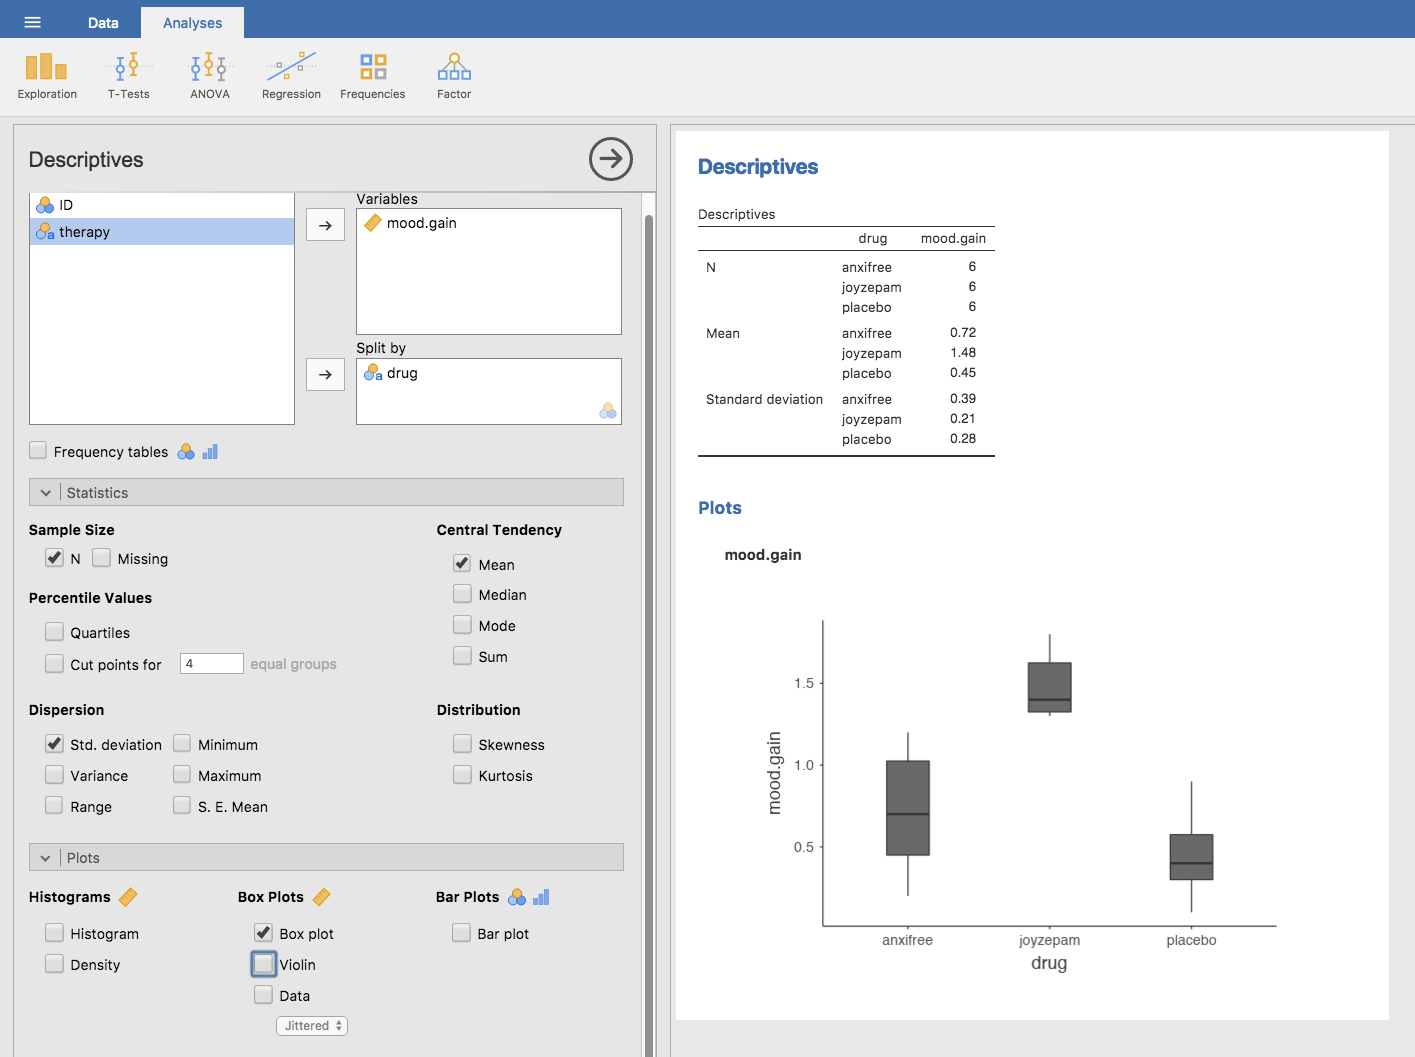
\epsfig{file = ../img/anova/anova1.png, clip=true,width = 14cm}
\caption{Descriptives for mood gain, and box plots by drug administered}
\HR
\label{fig:anova1}
\end{center}
\end{figure}

As the plot makes clear, there is a larger improvement in mood for participants in the Joyzepam group than for either the Anxifree group or the placebo group. The Anxifree group shows a larger mood gain than the control group, but the difference isn't as large. The question that we want to answer is are these difference ``real'', or are they just due to chance?


\section{How ANOVA works \label{sec:anovaintro}}

In order to answer the question posed by our clinical trial data we're going to run a one-way ANOVA. I'm going to start by showing you how to do it the hard way, building the statistical tool from the ground up and showing you how you could do it if you didn't have access to any of the cool built-in ANOVA functions in jamovi. And I hope you'll read it carefully, try to do it the long way once or twice to make sure you really understand how ANOVA works, and then once you've grasped the concept never {\it ever} do it this way again.

The experimental design that I described in the previous section strongly suggests that we're interested in comparing the average mood change for the three different drugs. In that sense, we're talking about an analysis similar to the $t$-test (Chapter~\ref{ch:ttest}) but involving more than two groups. If we let $\mu_P$ denote the population mean for the mood change induced by the placebo, and let $\mu_A$ and $\mu_J$ denote the corresponding means for our two drugs, Anxifree and Joyzepam, then the (somewhat pessimistic) null hypothesis that we want to test is that all three population means are identical. That is, {\it neither} of the two drugs is any more effective than a placebo. We can write out this null hypothesis as:
$$
\begin{array}{rcl}
H_0 &:& \mbox{it is true that } \mu_P = \mu_A = \mu_J
\end{array}
$$
As a consequence, our alternative hypothesis is that at least one of the three different treatments is different from the others. It's a bit tricky to write this mathematically, because (as we'll discuss) there are quite a few different ways in which the null hypothesis can be false. So for now we'll just write the alternative hypothesis like this:
$$
\begin{array}{rcl}
H_1 &:& \mbox{it is \underline{not} true that } \mu_P = \mu_A = \mu_J
\end{array}
$$
This null hypothesis is a lot trickier to test than any of the ones we've seen previously. How shall we do it? A sensible guess would be to ``do an ANOVA'', since that's the title of the chapter, but it's not particularly clear why an ``analysis of {\it variances}'' will help us learn anything useful about the {\it means}. In fact, this is one of the biggest conceptual difficulties that people have when first encountering ANOVA. To see how this works, I find it most helpful to start by talking about variances. In fact, what I'm going to do is start by playing some mathematical games with the formula that describes the variance. That is, we'll start out by playing around with variances and it will turn out that this gives us a useful tool for investigating means.

\SUBSECTION{Two formulas for the variance of \texorpdfstring{$Y$}{Y}}

First, let's start by introducing some notation. We'll use $G$ to refer to the total number of groups. For our data set there are three drugs, so there are $G=3$ groups. Next, we'll use $N$ to refer to the total sample size; there are a total of $N=18$ people in our data set. Similarly, let's use $N_k$ to denote the number of people in the $k$-th group. In our fake clinical trial, the sample size is $N_k = 6$ for all three groups.\FOOTNOTE{When all groups have the same number of observations, the experimental design is said to be ``balanced''. Balance isn't such a big deal for one-way ANOVA, which is the topic of this chapter. It becomes more important when you start doing more complicated ANOVAs.} Finally, we'll use $Y$ to denote the outcome variable. In our case, $Y$ refers to mood change. Specifically, we'll use $Y_{ik}$ to refer to the mood change experienced by the $i$-th member of the $k$-th group. Similarly, we'll use $\bar{Y}$ to be the average mood change, taken across all 18 people in the experiment, and $\bar{Y}_k$ to refer to the average mood change experienced by the 6 people in group $k$.  

\vspace{0.5cm}
\begin{mdframed}[style=MyFrame,nobreak=true]
Now that we've got our notation sorted out we can start writing down formulas. To start with, let's recall the formula for the variance that we used in Section~\ref{sec:var}, way back in those kinder days when we were just doing descriptive statistics. The sample variance of $Y$ is defined as follows
$$
\mbox{Var}(Y) = \frac{1}{N} \sum_{k=1}^G \sum_{i=1}^{N_k} \left(Y_{ik} - \bar{Y} \right)^2
$$
This formula looks pretty much identical to the formula for the variance in Section~\ref{sec:var}. The only difference is that this time around I've got two summations here: I'm summing over groups (i.e., values for $k$) and over the people within the groups (i.e., values for $i$). This is purely a cosmetic detail. If I'd instead used the notation $Y_p$ to refer to the value of the outcome variable for person $p$ in the sample, then I'd only have a single summation. The only reason that we have a double summation here is that I've classified people into groups, and then assigned numbers to people within groups. 
\end{mdframed}

A concrete example might be useful here. Let's consider this table, in which we have a total of $N=5$ people sorted into $G=2$ groups. Arbitrarily, let's say that the ``cool'' people are group 1 and the ``uncool'' people are group 2. It turns out that we have three cool people ($N_1 = 3$) and two uncool people ($N_2 = 2$)

\bigskip
\begin{center}
\begin{tabular}{lclccc} \hline 
name & person & group & group num. & index in group & grumpiness \\
& $p$ &          & $k$ & $i$ & $Y_{ik}$ or $Y_p$ \\ \hline
Ann & 1 & cool   &  1  &  1  & 20 \\
Ben & 2 & cool   &  1  &  2  & 55\\
Cat & 3 & cool   &  1  &  3  & 21\\
Dan & 4 & uncool &  2  &  1  & 91\\
Egg & 5 & uncool &  2  &  2  & 22\\
\end{tabular}
\end{center}
Notice that I've constructed two different labelling schemes here. We have a ``person'' variable $p$ so it would be perfectly sensible to refer to $Y_p$ as the grumpiness of the $p$-th person in the sample. For instance, the table shows that Dan is the fourth so we'd say $p = 4$. So, when talking about the grumpiness $Y$ of this ``Dan'' person, whoever he might be, we could refer to his grumpiness by saying that $Y_p = 91$, for person $p = 4$ that is.  However, that's not the only way we could refer to Dan. As an alternative we could note that Dan belongs to the ``uncool'' group ($k = 2$), and is in fact the first person listed in the uncool group ($i = 1$). So it's equally valid to refer to Dan's grumpiness by saying that $Y_{ik} = 91$, where $k = 2$ and $i = 1$. 

\vspace{0.5cm}
\begin{mdframed}[style=MyFrame,nobreak=true]
In other words, each person $p$ corresponds to a unique $ik$ combination, and so the formula that I gave above is actually identical to our original formula for the variance, which would be
$$
\mbox{Var}(Y) = \frac{1}{N} \sum_{p=1}^N  \left(Y_{p} - \bar{Y} \right)^2
$$
In both formulas, all we're doing is summing over all of the observations in the sample. Most of the time we would just use the simpler $Y_p$ notation; the equation using $Y_p$ is clearly the simpler of the two. However, when doing an ANOVA it's important to keep track of which participants belong in which groups, and we need to use the $Y_{ik}$ notation to do this. 
\end{mdframed}

\SUBSECTION{From variances to sums of squares}

Okay, now that we've got a good grasp on how the variance is calculated, let's define something called the \keyterm{total sum of squares}, which is denoted SS$_{tot}$. This is very simple. Instead of averaging the squared deviations, which is what we do when calculating the variance, we just add them up. 

\vspace{0.5cm}
\begin{mdframed}[style=MyFrame,nobreak=true]
So the formula for the total sum of squares is almost identical to the formula for the variance
$$
\mbox{SS}_{tot} = \sum_{k=1}^G \sum_{i=1}^{N_k} \left(Y_{ik} - \bar{Y} \right)^2
$$ 
\end{mdframed}
When we talk about analysing variances in the context of ANOVA, what we're really doing is working with the total sums of squares rather than the actual variance. One very nice thing about the total sum of squares is that we can break it up into two different kinds of variation. 

\vspace{0.5cm}
\begin{mdframed}[style=MyFrame,nobreak=true]
First, we can talk about the \keyterm{within-group sum of squares}, in which we look to see how different each individual person is from their own group mean
$$
\mbox{SS}_w = \sum_{k=1}^G \sum_{i=1}^{N_k} \left( Y_{ik} - \bar{Y}_k \right)^2
$$
where $\bar{Y}_k$ is a group mean. In our example, $\bar{Y}_k$ would be the average mood change experienced by those people given  the $k$-th drug. So, instead of comparing individuals to the average of \underline{all} people in the experiment, we're only comparing them to those people in the the same group. As a consequence, you'd expect the value of $\mbox{SS}_w$ to be smaller than the total sum of squares, because it's completely ignoring any group differences, i.e., whether the drugs will have different effects on people's moods.
\end{mdframed}
 
Next, we can define a third notion of variation which captures {\it only} the differences between groups. We do this by looking at the differences between the group means $\bar{Y}_k$ and grand mean $\bar{Y}$. 

\vspace{0.5cm}
\begin{mdframed}[style=MyFrame,nobreak=true]
In order to quantify the extent of this variation, what we do is calculate the \keyterm{between-group sum of squares}
\begin{eqnarray*}
\mbox{SS}_{b} &=& \sum_{k=1}^G \sum_{i=1}^{N_k} \left( \bar{Y}_k - \bar{Y} \right)^2 \\
&=& \sum_{k=1}^G N_k \left( \bar{Y}_k - \bar{Y} \right)^2
\end{eqnarray*}
\end{mdframed}

It's not too difficult to show that the total variation among people in the experiment $\mbox{SS}_{tot}$ is actually the sum of the differences between the groups $\mbox{SS}_b$ and the variation inside the groups $\mbox{SS}_w$. That is,
$$
\mbox{SS}_w  + \mbox{SS}_{b} = \mbox{SS}_{tot}
$$
Yay.


\begin{figure}
\begin{center}
\begin{tabular}{cc}
\epsfig{file = ../img/anova/anovaBetween.eps,clip=true, width = 7cm} & 
\epsfig{file = ../img/anova/anovaWithin.eps,clip=true, width = 7cm} \\
(a) & (b) 
\end{tabular}
\caption{Graphical illustration of ``between groups'' variation (panel a) and ``within groups'' variation (panel b). On the left the arrows show the differences in the group means. On the right the arrows highlight the variability within each group.}
\HR
\label{fig:anovavar}
\end{center}
\end{figure}

Okay, so what have we found out? We've discovered that the total variability associated with the outcome variable ($\mbox{SS}_{tot}$) can be mathematically carved up into the sum of ``the variation due to the differences in the sample means for the different groups'' ($\mbox{SS}_{b}$) plus ``all the rest of the variation'' ($\mbox{SS}_{w}$)\FOOTNOTE{$\mbox{SS}_{w}$ is also referred to in an independent ANOVA as the error variance, or $\mbox{SS}_{error}$}. How does that help me find out whether the groups have different population means? Um. Wait. Hold on a second. Now that I think about it, this is {\it exactly} what we were looking for. If the null hypothesis is true then you'd expect all the sample means to be pretty similar to each other, right? And that would imply that you'd expect $\mbox{SS}_{b}$ to be really small, or at least you'd expect it to be a lot smaller than ``the variation associated with everything else'', $\mbox{SS}_{w}$. Hmm. I detect a hypothesis test coming on.

\SUBSECTION{From sums of squares to the \texorpdfstring{$F$}{F}-test}

As we saw in the last section, the {\it qualitative} idea behind ANOVA is to compare the two sums of squares values $\mbox{SS}_b$ and $\mbox{SS}_w$ to each other. If the between-group variation $\mbox{SS}_b$ is large relative to the within-group variation $\mbox{SS}_w$ then we have reason to suspect that the population means for the different groups aren't identical to each other. In order to convert this into a workable hypothesis test, there's a little bit of ``fiddling around'' needed. What I'll do is first show you {\it what} we do to calculate our test statistic, the \keyterm{$F$ ratio}, and then try to give you a feel for {\it why} we do it this way. 

In order to convert our SS values into an $F$-ratio the first thing we need to calculate is the \keyterm{degrees of freedom} associated with the SS$_b$ and SS$_w$ values. As usual, the degrees of freedom corresponds to the number of unique ``data points'' that contribute to a particular calculation, minus the number of ``constraints'' that they need to satisfy. For the within-groups variability what we're calculating is the variation of the individual observations ($N$ data points) around the group means ($G$ constraints). In contrast, for the between groups variability we're interested in the variation of the group means ($G$ data points) around the grand mean (1 constraint). Therefore, the degrees of freedom here are:
$$
\begin{array}{lcl}
\mbox{df}_b &=& G-1 \\
\mbox{df}_w &=& N-G \\
\end{array}
$$
Okay, that seems simple enough. What we do next is convert our summed squares value into a ``mean squares'' value, which we do by dividing by the degrees of freedom: 
$$
\begin{array}{lcl}
\mbox{MS}_b &=& \displaystyle\frac{\mbox{SS}_b }{ \mbox{df}_b} \vspace*{6pt} \\
\mbox{MS}_w &=& \displaystyle\frac{\mbox{SS}_w }{ \mbox{df}_w} 
\end{array}
$$
Finally, we calculate the $F$-ratio by dividing the between-groups MS by the within-groups MS:
$$
F = \frac{\mbox{MS}_b }{ \mbox{MS}_w } 
$$
At a very general level, the intuition behind the $F$ statistic is straightforward. Bigger values of $F$ means that the between-groups variation is large relative to the within-groups variation. As a consequence, the larger the value of $F$ the more evidence we have against the null hypothesis. But how large does $F$ have to be in order to actually {\it reject} $H_0$? In order to understand this, you need a slightly deeper understanding of what ANOVA is and what the mean squares values actually are. 

The next section discusses that in a bit of detail, but for readers that aren't interested in the details of what the test is actually measuring I'll cut to the chase. In order to complete our hypothesis test we need to know the sampling distribution for $F$ if the null hypothesis is true. Not surprisingly, the sampling distribution for the $F$ \underline{statistic} under the null hypothesis is an $F$ \underline{distribution}. If you recall our discussion of the $F$ distribution in Chapter~\ref{ch:probability}, the $F$ distribution has two parameters, corresponding to the two degrees of freedom involved. The first one df$_1$ is the between groups degrees of freedom df$_b$, and the second one df$_2$ is the within groups degrees of freedom df$_w$. 

A summary of all the key quantities involved in a one-way ANOVA, including the formulas showing how they are calculated, is shown in Table~\ref{tab:anovatable}. 

\begin{table}
\begin{center}
\caption{All of the key quantities involved in an ANOVA organised into a ``standard'' ANOVA table. The formulas for all quantities (except the $p$-value which has a very ugly formula and would be nightmarishly hard to calculate without a computer) are shown.} 

\tabcapsep
\label{tab:anovatable}
\small
\begin{tabular}{p{1.8cm}|c|c|c|c|c} 
& df & sum of squares & mean squares & $F$-statistic & $p$-value \\  \hline  &&&&& \\ 
\raggedright
between groups & $\mbox{df}_b = G-1$ & SS$_b = \displaystyle\sum_{k=1}^G N_k (\bar{Y}_k - \bar{Y})^2$ & $\mbox{MS}_b = \displaystyle\frac{\mbox{SS}_b}{\mbox{df}_b}$ & $ F = \displaystyle\frac{\mbox{MS}_b }{ \mbox{MS}_w }$ & [complicated] \\ &&&&&\\ 
\raggedright
within groups   & $\mbox{df}_w = N-G$ & SS$_w = \displaystyle\sum_{k=1}^G \displaystyle\sum_{i = 1}^{N_k} ( {Y}_{ik} - \bar{Y}_k)^2$ & $\mbox{MS}_w =  \displaystyle\frac{\mbox{SS}_w}{\mbox{df}_w}$ & - & - \\ 
\end{tabular}
\tabcapsep
\HR
\end{center}
\end{table}

\vspace{0.5cm}
\begin{mdframed}[style=MyFrame,nobreak=false]
\SUBSECTION{The model for the data and the meaning of \texorpdfstring{$F$}{F} \advanced\label{sec:anovamodel}}

At a fundamental level ANOVA is a competition between two different statistical models, $H_0$ and $H_1$. When I described the null and alternative hypotheses at the start of the section, I was a little imprecise about what these models actually are. I'll remedy that now, though you probably won't like me for doing so. If you recall, our null hypothesis was that all of the group means are identical to one another. If so, then a natural way to think about the outcome variable $Y_{ik}$ is to describe individual scores in terms of a single population mean $\mu$, plus the deviation from that population mean. This deviation is usually denoted $\epsilon_{ik}$ and is traditionally called the {\it error} or \keyterm{residual} associated with that observation. Be careful though. Just like we saw with the word ``significant'', the word ``error'' has a technical meaning in statistics that isn't quite the same as its everyday English definition. In everyday language, ``error'' implies a mistake of some kind, but in statistics it doesn't (or at least, not necessarily). With that in mind, the word ``residual'' is a better term than the word ``error''. In statistics both words mean ``leftover variability'', that is ``stuff'' that the model can't explain. 

In any case, here's what the null hypothesis looks like when we write it as a statistical model
$$
Y_{ik} = \mu + \epsilon_{ik}
$$
where we make the {\it assumption} (discussed later) that the residual values $\epsilon_{ik}$ are normally distributed, with mean 0 and a standard deviation $\sigma$ that is the same for all groups. To use the notation that we introduced in Chapter~\ref{ch:probability} we would write this assumption like this
$$
\epsilon_{ik} \sim \mbox{Normal}(0, \sigma^2)
$$

What about the alternative hypothesis, $H_1$? The only difference between the null hypothesis and the alternative hypothesis is that we allow each group to have a different population mean. So, if we let $\mu_k$ denote the population mean for the $k$-th group in our experiment, then the statistical model corresponding to $H_1$ is
$$
Y_{ik} = \mu_k + \epsilon_{ik}
$$
where, once again, we assume that the error terms are normally distributed with mean 0 and standard deviation $\sigma$. That is, the alternative hypothesis also assumes that 
$
\epsilon \sim \mbox{Normal}(0, \sigma^2)
$

Okay, now that we've described the statistical models underpinning $H_0$ and $H_1$ in more detail, it's now pretty straightforward to say what the mean square values are measuring, and what this means for the interpretation of $F$. I won't bore you with the proof of this but it turns out that the within-groups mean square, MS$_w$, can be viewed as an estimator (in the technical sense, Chapter~\ref{ch:estimation}) of the error variance $\sigma^2$. The between-groups mean square MS$_b$ is also an estimator, but what it estimates is the error variance {\it plus} a quantity that depends on the true differences among the group means. If we call this quantity $Q$, then we can see that the $F$-statistic is basically\FOOTNOTE{If you read ahead to Chapter~\ref{ch:anova2} and look at how the ``treatment effect'' at level $k$ of a factor is defined in terms of the $\alpha_k$ values (see Section~\ref{sec:interactions}), it turns out that $Q$ refers to a weighted mean of the squared treatment effects, $Q=(\sum_{k=1}^G N_k \alpha_k^2)/(G-1)$. }
$$
F = \frac{\hat{Q} + \hat\sigma^2}{\hat\sigma^2}
$$
where the true value $Q=0$ if the null hypothesis is true, and $Q > 0$ if the alternative hypothesis is true \parencite[e.g.,][ch.\ 10]{Hays1994}. Therefore, at a bare minimum {\it the $F$ value must be larger than 1} to have any chance of rejecting the null hypothesis. Note that this {\it doesn't} mean that it's impossible to get an $F$-value less than 1. What it means is that if the null hypothesis is true the sampling distribution of the $F$ ratio has a mean of 1,\FOOTNOTE{Or, if we want to be sticklers for accuracy, $1 + \frac{2}{df_2 - 2}$.} and so we need to see $F$-values larger than 1 in order to safely reject the null.

To be a bit more precise about the sampling distribution, notice that if the null hypothesis is true, both MS$_b$ and MS$_w$ are estimators of the variance of the residuals $\epsilon_{ik}$. If those residuals are normally distributed, then you might suspect that the estimate of the variance of $\epsilon_{ik}$ is chi-square distributed, because (as discussed in Section~\ref{sec:otherdists}) that's what a chi-square distribution {\it is}: it's what you get when you square a bunch of normally-distributed things and add them up. And since the $F$ distribution is (again, by definition) what you get when you take the ratio between two things that are $\chi^2$ distributed, we have our sampling distribution. Obviously, I'm glossing over a whole lot of stuff when I say this, but in broad terms, this really is where our sampling distribution comes from. %\TODO {\bf [CITE]}
\end{mdframed}

\SUBSECTION{A worked example \label{sec:anovacalc}}

% `\TODO {\bf recheck all the numbers here}
The previous discussion was fairly abstract and a little on the technical side, so I think that at this point it might be useful to see a worked example. For that, let's go back to the clinical trial data that I introduced at the start of the chapter. The descriptive statistics that we calculated at the beginning tell us our group means: an average mood gain of 0.45 for the placebo, 0.72 for Anxifree, and 1.48 for Joyzepam. With that in mind, let's party like it's 1899 \FOOTNOTE{Or, to be precise, party like ``it's 1899 and we've got no friends and nothing better to do with our time than do some calculations that wouldn't have made any sense in 1899 because ANOVA didn't exist until about the 1920s''.} and  start doing some pencil and paper calculations. I'll only do this for the first 5 observations because it's not bloody 1899 and I'm very lazy. Let's start by calculating $\mbox{SS}_{w}$, the within-group sums of squares. First, let's draw up a nice table to help us with our calculations: 

\small
\vspace*{6pt}
%\begin{center}
\begin{tabular}{c|c} %{c|c|c|c|c}
{group} & {outcome}  \\ %& group mean & deviation from group mean & squared deviation\\  
  $k$ &  $Y_{ik}$ \\ \hline % & $\bar{Y}_k$ & $Y_{ik} - \bar{Y}_{k}$ &  $(Y_{ik} - \bar{Y}_{k})^2$\\  \hline
{placebo}  & {0.5}  \\% &   &  & \\
{placebo}  & {0.3} \\% &   &  & \\
{placebo}  &  {0.1}\\% &   &  & \\
{anxifree}  & {0.6} \\% &   &  & \\
{anxifree}  & {0.4}\\% &   &  & \\ 
\end{tabular}
%\end{center}
\vspace*{6pt}
\normalsize

\noindent
At this stage, the only thing I've included in the table is the raw data itself. That is, the grouping variable (i.e., \rtext{drug}) and outcome variable (i.e. \rtext{mood.gain}) for each person. Note that the outcome variable here corresponds to the $Y_{ik}$ value in our equation previously. The next step in the calculation is to write down, for each person in the study, the corresponding group mean, $\bar{Y}_k$. This is slightly repetitive but not particularly difficult since we already calculated those group means when doing our descriptive statistics:

\small
\vspace*{6pt}
%\begin{center}
\begin{tabular}{c|c|c} %|c|c}
 group & outcome  & {\bf group mean} \\% & deviation from group mean & squared deviation\\  
  $k$ &  $Y_{ik}$  & $\bar{Y}_k$ \\ \hline % & $Y_{ik} - \bar{Y}_{k}$ &  $(Y_{ik} - \bar{Y}_{k})^2$\\  \hline
placebo  & 0.5  & {\bf 0.45} \\% &  & \\
placebo  & 0.3 &  {\bf 0.45} \\%&  & \\
placebo  &  0.1 &  {\bf 0.45} \\%&  & \\
anxifree  & 0.6  & {\bf 0.72} \\% &  & \\
anxifree  &  0.4 &  {\bf 0.72}\\% &  & \\ 
\end{tabular}
%\end{center}
\vspace*{6pt}
\normalsize

\noindent
Now that we've written those down, we need to calculate, again for every person, the deviation from the corresponding group mean. That is, we want to subtract $Y_{ik} - \bar{Y}_k$. After we've done that, we need to square everything. When we do that, here's what we get:

\small
\vspace*{6pt}
%\begin{center}
\begin{tabular}{c|c|c|c|c}
 group & outcome  & group mean & {\bf dev.\ from group mean} & {\bf squared deviation}\\  
  $k$ &  $Y_{ik}$  & $\bar{Y}_k$ & $Y_{ik} - \bar{Y}_{k}$ &  $(Y_{ik} - \bar{Y}_{k})^2$\\  \hline
placebo  & 0.5  & 0.45  & {\bf 0.05}  & {\bf 0.0025} \\
placebo  & 0.3 &  0.45 &  {\bf -0.15} & {\bf 0.0225}\\
placebo  &  0.1 &  0.45 &{\bf -0.35}  & {\bf 0.1225} \\
anxifree  & 0.6  & 0.72  & {\bf -0.12}  & {\bf 0.0136} \\
anxifree  &  0.4 &  0.72 & {\bf -0.32} & {\bf 0.1003} \\ 
\end{tabular}
%\end{center}
\vspace*{6pt}
\normalsize

\noindent
The last step is equally straightforward. In order to calculate the within-group sum of squares we just add up the squared deviations across all observations:
$$
\begin{array}{rcl}
\mbox{SS}_w &=& 0.0025 + 0.0225 + 0.1225 + 0.0136 + 0.1003 \\
&=& 0.2614
\end{array}
$$
\noindent
Of course, if we actually wanted to get the {\it right} answer we'd need to do this for all 18 observations in the data set, not just the first five. We could continue with the pencil and paper calculations if we wanted to, but it's pretty tedious. Alternatively, it's not too hard to do this in a dedicated spreadsheet programme such as OpenOffice or Excel. Try and do it yourself. The one that I did, in Excel, is in the file \filename{clinicaltrial\_anova.xls}. When you do it you should end up with a within-group sum of squares value of 1.39. 

Okay. Now that we've calculated the within groups variation, $\mbox{SS}_w$, it's time to turn our attention to the between-group sum of squares, $\mbox{SS}_b$. The calculations for this case are very similar. The main difference is that instead of calculating the differences between an observation $Y_{ik}$ and a group mean $\bar{Y}_k$ for all of the observations, we calculate the differences between the group means $\bar{Y}_k$ and the grand mean $\bar{Y}$ (in this case 0.88) for all of the groups. 

\small
\vspace*{6pt}
%\begin{center}
\begin{tabular}{c|c|c|c|c}
 group & group mean  & grand mean & deviation               & squared deviations \\  
  $k$  & $\bar{Y}_k$ & $\bar{Y}$  & $\bar{Y}_{k} - \bar{Y}$ & $(\bar{Y}_{k} - \bar{Y})^2$ \\  \hline
placebo   & 0.45  &  0.88 &  -0.43 &  0.19 \\
anxifree  & 0.72  &  0.88 &  -0.16 &  0.03 \\
joyzepam  & 1.48  &  0.88 &  0.60  &  0.36 \\
\end{tabular}
%\end{center}
\vspace*{6pt}
\normalsize

\noindent
However, for the between group calculations we need to multiply each of these squared deviations by $N_k$, the number of observations in the group. We do this because every {\it observation} in the group (all $N_k$ of them) is associated with a between group difference. So if there are six people in the placebo group and the placebo group mean differs from the grand mean by 0.19, then the {\it total} between group variation associated with these six people is $6 \times 0.19 = 1.14$. So we have to extend our little table of calculations:

\small
%\begin{center}
\vspace*{6pt}
\begin{tabular}{c|c |c|c|c}
 group & \hspace{.25cm}...\hspace{.25cm} & squared deviations & sample size & weighted squared dev\\  
  $k$  & ... & $(\bar{Y}_{k} - \bar{Y})^2$ & $N_k$ & $N_k (\bar{Y}_{k} - \bar{Y})^2$\\  \hline
placebo   & ... &  0.19 & 6 & 1.14\\
anxifree  & ... &  0.03 & 6 & 0.18\\
joyzepam  & ... &  0.36 & 6 & 2.16\\
\end{tabular}
%\end{center}
\vspace*{6pt}
\normalsize

\noindent
And so now our between group sum of squares is obtained by summing these ``weighted squared deviations'' over all three groups in the study:
$$
\begin{array}{rcl}
\mbox{SS}_{b} &=& 1.14 + 0.18 + 2.16 \\
&=& 3.48
\end{array}
$$
As you can see, the between group calculations are a lot shorter\FOOTNOTE{In the Excel \filename{clinicaltrial\_anova.xls} the value for $SS_b$ worked out to be very slightly different, 3.45, than that shown in the text above (rounding errors!)}. Now that we've calculated our sums of squares values, $\mbox{SS}_b$ and $\mbox{SS}_w$, the rest of the ANOVA is pretty painless. The next step is to calculate the degrees of freedom. Since we have $G = 3$ groups and $N = 18$ observations in total our degrees of freedom can be calculated by simple subtraction:
$$
\begin{array}{lclcl}
\mbox{df}_b &=& G - 1 &=& 2 \\
\mbox{df}_w &=& N - G &=& 15 
\end{array}
$$
Next, since we've now calculated the values for the sums of squares and the degrees of freedom, for both the within-groups variability and the between-groups variability, we can obtain the mean square values by dividing one by the other:
$$
\begin{array}{lclclcl}
\mbox{MS}_b &=& \displaystyle\frac{\mbox{SS}_b }{  \mbox{df}_b } &=& \displaystyle\frac{3.48}{ 2}  &=& 1.74 \vspace*{6pt} \\ 
\mbox{MS}_w &=& \displaystyle\frac{\mbox{SS}_w }{  \mbox{df}_w } &=& \displaystyle\frac{1.39}{15} &=& 0.09
\end{array}
$$
We're almost done. The mean square values can be used to calculate the $F$-value, which is the test statistic that we're interested in. We do this by dividing the between-groups MS value by the within-groups MS value.
$$
F \ = \ \frac{\mbox{MS}_b }{ \mbox{MS}_w } \ = \ \frac{1.74}{0.09} \ = \ 19.3
$$
Woohooo! This is terribly exciting, yes? Now that we have our test statistic, the last step is to find out whether the test itself gives us a significant result. As discussed in Chapter~\ref{ch:hypothesistesting} back in the ``old days'' what we'd do is open up a statistics textbook or flick to the back section which would actually have a huge lookup table and we would find the threshold $F$ value corresponding to a particular value of alpha (the null hypothesis rejection region), e.g. 0.05, 0.01 or 0.001, for 2 and 15 degrees of freedom. Doing it this way would give us a threshold $F$ value for an alpha of 0.001 of 11.34. As this is less than our calculated $F$ value we say that $p < 0.001$. But those were the old days, and nowadays fancy stats software calculates the exact $p$-value for you. In fact, the exact $p$-value is 0.000071. So, unless we're being {\it extremely} conservative about our Type I error rate, we're pretty much guaranteed to reject the null hypothesis. 

At this point, we're basically done. Having completed our calculations, it's traditional to organise all these numbers into an ANOVA table like the one in Table~\ref{tab:anovatable}. For our clinical trial data, the ANOVA table would look like this:
\begin{center}
\begin{tabular}{l|ccccc} 
& df & sum of squares & mean squares & $F$-statistic & $p$-value \\  \hline 
between groups & 2 & 3.48 & 1.74 & 19.3 & 0.000071 \\
within groups   & 15 & 1.39 & 0.09 & - & - \\ 
\end{tabular}
\end{center}
\noindent
These days, you'll probably never have much reason to want to construct one of these tables yourself, but you \underline{will} find that almost all statistical software (jamovi included) tends to organise the output of an ANOVA into a table like this, so it's a good idea to get used to reading them. However, although the software will output a full ANOVA table, there's almost never a good reason to include the whole table in your write up. A pretty standard way of reporting this result would be to write something like this:
\begin{quote}
One-way ANOVA showed a significant effect of drug on mood gain ($F(2,15) = 19.3, p<.001$).
\end{quote}
Sigh. So much work for one short sentence.


\section{Running an ANOVA in jamovi\label{sec:introduceaov}}

I'm pretty sure I know what you're thinking after reading the last section, {\it especially} if you followed my advice and did all of that by pencil and paper (i.e., in a spreadsheet) yourself. Doing the ANOVA calculations yourself {\it sucks}. There's quite a lot of calculations that we needed to do along the way, and it would be tedious to have to do this over and over again every time you wanted to do an ANOVA. 

\SUBSECTION{Using jamovi to specify your ANOVA}

To make life easier for you, jamovi can do ANOVA..hurrah! Go to the `ANOVA' - `ANOVA' analysis, and move the \rtext{mood.gain} variable across so it is in the `Dependent Variable' box, and then move the \rtext{drug} variable across so it is in the `Fixed Factors' box. This should give the results as shown in Figure \ref{fig:anova2}. \FOOTNOTE{The jamovi results are more accurate than the ones in the text above, due to rounding errors.} Note I have also checked the $\eta^2$ checkbox, pronounced ``eta'' squared, under the `Effect Size' option and this is also shown on the results table. We will come back to effect sizes a bit later.

\begin{figure}[htb]
\begin{center}
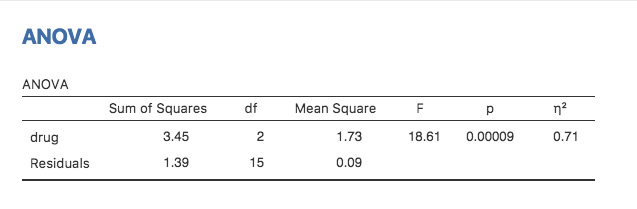
\epsfig{file = ../img/anova/anova2.png, clip=true,width = 14cm}
\caption{jamovi results table for ANOVA of mood gain by drug administered}
\HR
\label{fig:anova2}
\end{center}
\end{figure}

The jamovi results table shows you the sums of squares values, the degrees of freedom, and a couple of other quantities that we're not really interested in right now. Notice, however, that jamovi doesn't use the names ``between-group'' and ``within-group''. Instead, it tries to assign more meaningful names. In our particular example, the {\it between groups} variance corresponds to the effect that the \rtext{drug} has on the outcome variable, and the {\it within groups} variance corresponds to the ``leftover'' variability so it calls that the {\it residuals}. If we compare these numbers to the numbers that I calculated by hand in Section~\ref{sec:anovacalc}, you can see that they're more or less the same, apart from rounding errors. The between groups sums of squares is $\mbox{SS}_b = 3.45$, the within groups sums of squares is $\mbox{SS}_w = 1.39$, and the degrees of freedom are 2 and 15 respectively. We also get the $F$-value and the $p$-value and, again, these are more or less the same, give or take rounding errors, to the numbers that we calculated ourselves when doing it the long and tedious way. 


\section{Effect size\label{sec:etasquared}}

There's a few different ways you could measure the effect size in an ANOVA, but the most commonly used measures are $\eta^2$ (\keyterm{eta squared}) and partial $\eta^2$. For a one way analysis of variance they're identical to each other, so for the moment I'll just explain $\eta^2$. The definition of $\eta^2$ is actually really simple
$$
\eta^2 = \frac{\mbox{SS}_b}{\mbox{SS}_{tot}}
$$
That's all it is. So when I look at the ANOVA table in Figure~\ref{fig:anova2}, I see that $\mbox{SS}_b = 3.45$  and $\mbox{SS}_{tot} = 3.45 + 1.39 = 4.84$. Thus we get an $\eta^2$ value of 
$$
\eta^2 = \frac{3.45}{4.84} = 0.71
$$
The interpretation of $\eta^2$ is equally straightforward. It refers to the proportion of the variability in the outcome variable (\rtext{mood.gain}) that can be explained in terms of the predictor (\rtext{drug}). A value of $\eta^2 = 0$ means that there is no relationship at all between the two, whereas a value of $\eta^2 = 1$ means that the relationship is perfect. Better yet, the $\eta^2$ value is very closely related to $R^2$, as discussed previously in Section \ref{sec:rsquared}), and has an equivalent interpretation.

Although many statistics text books suggest $\eta^2$ as the default effect size measure in ANOVA, there's an interesting blog post by Daniel Lakens suggesting that eta-squared is perhaps not the best measure of effect size in real world data analysis, because it can be a biased estimator (\url{http://daniellakens.blogspot.com.au/2015/06/why-you-should-use-omega-squared.html}). Usefully, there is also an option in jamovi to specify omega-squared ($\omega^2$), which is less biased, alongside eta-squared.


\section{Multiple comparisons and post hoc tests~\label{sec:posthoc}}

%Holm, S. (1979). A simple sequentially rejective multiple test procedure. Scandinavian Journal of Statistics, 6, 65-70.
%Shaffer, J. P. (1995). Multiple Hypothesis Testing. Annual Review of Psych., 46, 561-584.


% Read Hsu (1996).

%%%%%%%%%%%%%%%%%%%%%

% Notes from Sahai & Ageel:
%
% pairwise 
%    + balanced design ---> Tukey
%    + unbalanced ---> Tukey Kramer
%
% not pairwise tests
%     + there's a control group --> Dunnett
%     + planned --> Bonferroni
%     + not planned --> Scheffe

%%%%%%%%%%%%%%%%%%%%%

Any time you run an ANOVA with more than two groups and you end up with a significant effect, the first thing you'll probably want to ask is which groups are actually different from one another. In our drugs example, our null hypothesis was that all three drugs (placebo, Anxifree and Joyzepam) have the exact same effect on mood. But if you think about it, the null hypothesis is actually claiming {\it three} different things all at once here. Specifically, it claims that:
\begin{itemize} \itemsep 0pt
\item Your competitor's drug (Anxifree) is no better than a placebo (i.e., $\mu_A = \mu_P$)
\item Your drug (Joyzepam) is no better than a placebo (i.e., $\mu_J = \mu_P$)
\item Anxifree and Joyzepam are equally effective (i.e., $\mu_J = \mu_A$)
\end{itemize}
If any one of those three claims is false, then the null hypothesis is also false. So, now that we've rejected our null hypothesis, we're thinking that {\it at least} one of those things isn't true. But which ones? All three of these propositions are of interest. Since you certainly want to know if your new drug Joyzepam is better than a placebo, it would be nice to know how well it stacks up against an existing commercial alternative (i.e., Anxifree). It would even be useful to check the performance of Anxifree against the placebo. Even if Anxifree has already been extensively tested against placebos by other researchers, it can still be very useful to check that your study is producing similar results to earlier work.

When we characterise the null hypothesis in terms of these three distinct propositions, it becomes clear that there are eight possible ``states of the world'' that we need to distinguish between:
\begin{center}
\begin{tabular}{c|ccc|c}
possibility: & is $\mu_P = \mu_A$? & is $\mu_P = \mu_J$? & is $\mu_A = \mu_J$? & which hypothesis?\\ \hline
1 & \checkmark & \checkmark & \checkmark & null \\
2 & \checkmark & \checkmark &  & alternative \\
3 & \checkmark & & \checkmark & alternative \\
4 & \checkmark & & & alternative \\
5 & & \checkmark & \checkmark & alternative \\
6 & & \checkmark & & alternative \\
7 & & & \checkmark & alternative \\
8 & & & & alternative \\
\end{tabular}
\end{center}
By rejecting the null hypothesis, we've decided that we {\it don't} believe that \#1 is the true state of the world. The next question to ask is, which of the other seven possibilities {\it do} we think is right? When faced with this situation, its usually helps to look at the data. For instance, if we look at the plots in Figure~\ref{fig:anova1}, it's tempting to conclude that Joyzepam is better than the placebo and better than Anxifree, but there's no real difference between Anxifree and the placebo. However, if we want to get a clearer answer about this, it might help to run some tests. 

\SUBSECTION{Running ``pairwise'' \texorpdfstring{$t$}{t}-tests}

How might we go about solving our problem? Given that we've got three separate pairs of means (placebo versus Anxifree, placebo versus Joyzepam, and Anxifree versus Joyzepam) to compare, what we could do is run three separate $t$-tests and see what happens. This is easy to do in jamovi. Go to the ANOVA `Post Hoc Tests' options, move the `drug' variable across into the active box on the right, and then click on the `No correction' checkbox. This will produce a neat table showing all the pairwise $t$-test comparisons  amongst the three levels of the \rtext{drug} variable, as in Figure \ref{fig:anova3}.

\begin{figure}[htb]
\begin{center}
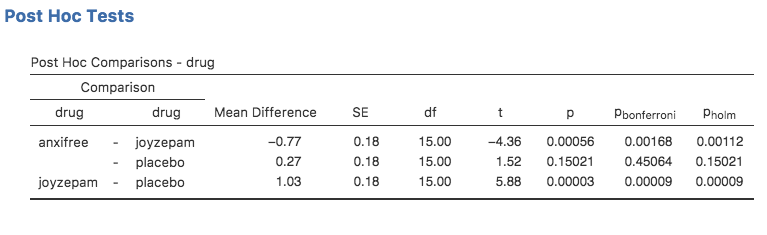
\epsfig{file = ../img/anova/anova3.png, clip=true,width = 14cm}
\caption{Uncorrected pairwise $t$-tests as post hoc comparisons in jamovi}
\HR
\label{fig:anova3}
\end{center}
\end{figure}

\SUBSECTION{Corrections for multiple testing}

In the previous section I hinted that there's a problem with just running lots and lots of $t$-tests. The concern is that, when running these analyses, what we're doing is going on a ``fishing expedition''. We're running lots and lots of tests without much theoretical guidance in the hope that some of them come up significant. This kind of theory-free search for group differences is referred to as \keyterm{post hoc analysis} (``post hoc'' being Latin for ``after this'').\FOOTNOTE{If you {\it do} have some theoretical basis for wanting to investigate some comparisons but not others, it's a different story. In those circumstances you're not really running ``post hoc'' analyses at all, you're making ``planned comparisons''. I do talk about this situation later in the book (Section~\ref{sec:plannedcomparisons}), but for now I want to keep things simple.}   

It's okay to run post hoc analyses, but a lot of care is required. For instance, the analysis that I ran in the previous section should be avoided, as each {\it individual} $t$-test is designed to have a 5\% Type I error rate (i.e., $\alpha = .05$) and I ran three of these tests. Imagine what would have happened if my ANOVA involved 10 different groups, and I had decided to run 45 ``post hoc'' $t$-tests to try to find out which ones were significantly different from each other, you'd expect 2 or 3 of them to come up significant {\it by chance alone}. As we saw in Chapter~\ref{ch:hypothesistesting}, the central organising principle behind null hypothesis testing is that we seek to control our Type I error rate, but now that I'm running lots of $t$-tests at once in order to determine the source of my ANOVA results, my actual Type I error rate across this whole {\it family} of tests has gotten completely out of control. 

The usual solution to this problem is to introduce an adjustment to the $p$-value, which aims to control the total error rate across the family of tests \parencite[see][]{Shaffer1995}. An adjustment of this form, which is usually (but not always) applied because one is doing post hoc analysis, is often referred to as a \keyterm{correction for multiple comparisons}, though it is sometimes referred to as ``simultaneous inference''. In any case, there are quite a few different ways of doing this adjustment. I'll discuss a few of them in this section and in Section~\ref{sec:posthoc2}, but you should be aware that there are many other methods out there \parencite[see, e.g.,][]{Hsu1996}. 

\SUBSECTION{Bonferroni corrections}

The simplest of these adjustments is called the \keyterm{Bonferroni correction} \parencite{Dunn1961}, and it's very very simple indeed. Suppose that my post hoc analysis consists of $m$ separate tests, and I want to ensure that the total probability of making {\it any} Type I errors at all is at most $\alpha$.\FOOTNOTE{It's worth noting in passing that not all adjustment methods try to do this. What I've described here is an approach for controlling ``family wise Type I error rate''. However, there are other post hoc tests that seek to control the ``false discovery rate'', which is a somewhat different thing.} If so, then the Bonferroni correction just says ``multiply all your raw $p$-values by $m$''. If we let $p$ denote the original $p$-value, and let $p^\prime_j$ be the corrected value, then the Bonferroni correction tells that:
$$
p^\prime = m \times p
$$
And therefore, if you're using the Bonferroni correction, you would reject the null hypothesis if $p^\prime < \alpha$. The logic behind this correction is very straightforward. We're doing $m$ different tests, so if we arrange it so that each test has a Type I error rate of at most $\alpha / m$, then the {\it total} Type I error rate across these tests cannot be larger than $\alpha$. That's pretty simple, so much so that in the original paper, the author writes,
\begin{quote}
The method given here is so simple and so general that I am sure it must have been used before this. I do not find it, however, so can only conclude that perhaps its very simplicity has kept statisticians from realizing that it is a very good method in some situations \parencite[pp 52-53]{Dunn1961}
\end{quote}
To use the Bonferroni correction in jamovi, just click on the `Bonferroni' checkbox in the `Correction' options, and you will see another column added to the ANOVA results table showing the adjusted $p$-values for the Bonferroni correction (\ref{fig:anova3}). If we compare these three $p$-values to those for the uncorrected, pairwise $t$-tests, it is clear that the only thing that jamovi has done is multiply them by 3. 

\SUBSECTION{Holm corrections}

Although the Bonferroni correction is the simplest adjustment out there, it's not usually the best one to use. One method that is often used instead is the \keyterm{Holm correction} \parencite{Holm1979}. The idea behind the Holm correction is to pretend that you're doing the tests sequentially, starting with the smallest (raw) $p$-value and moving onto the largest one. For the $j$-th largest of the $p$-values, the adjustment is {\it either}
$$
p^\prime_j = j \times p_j 
$$
(i.e., the biggest $p$-value remains unchanged, the second biggest $p$-value is doubled, the third biggest $p$-value is tripled, and so on), {\it or}
$$
p^\prime_j = p^\prime_{j+1}
$$
whichever one is \underline{larger}. This might sound a little confusing, so let's go through it a little more slowly. Here's what the Holm correction does. First, you sort all of your $p$-values in order, from smallest to largest. For the smallest $p$-value all you do is multiply it by $m$, and you're done. However, for all the other ones it's a two-stage process. For instance, when you move to the second smallest $p$ value, you first multiply it by $m-1$. If this produces a number that is bigger than the adjusted $p$-value that you got last time, then you keep it. But if it's smaller than the last one, then you copy the last $p$-value. To illustrate how this works, consider the table below, which shows the calculations of a Holm correction for a collection of five $p$-values:
\begin{center}
\begin{tabular}{rrrr} 
 raw $p$ & rank $j$ & $p \times j$ & Holm $p$   \\ \hline
.001 & 5 & .005 & .005 \\
.005 & 4 & .020 & .020 \\
.019 & 3 & .057 & .057 \\
.022 & 2 & .044 & .057 \\
.103 & 1 & .103 & .103 \\
\end{tabular}
\end{center}
Hopefully that makes things clear. 

Although it's a little harder to calculate, the Holm correction has some very nice properties. It's more powerful than Bonferroni (i.e., it has a lower Type II error rate) but, counter-intuitive as it might seem, it has the {\it same} Type I error rate. As a consequence, in practice there's never any reason to use the simpler Bonferroni correction since it is always outperformed by the slightly more elaborate Holm correction. Because of this, the Holm correction should be your {\it go to} multiple comparison correction. Figure \ref{fig:anova3} also shows the Holm corrected $p$-values and, as you can see, the biggest $p$-value (corresponding to the comparison between Anxifree and the placebo) is unaltered. At a value of $.15$, it is exactly the same as the value we got originally when we applied no correction at all. In contrast, the smallest $p$-value (Joyzepam versus placebo) has been multiplied by three. 

\SUBSECTION{Writing up the post hoc test}

Finally, having run the post hoc analysis to determine which groups are significantly different to one another, you might write up the result like this:
\begin{quote}
Post hoc tests (using the Holm correction to adjust $p$) indicated that Joyzepam produced a significantly larger mood change than both Anxifree ($p = .001$) and the placebo ($p = 9.0 \times 10^{-5}$). We found no evidence that Anxifree performed better than the placebo ($p = .15$).
\end{quote}
Or, if you don't like the idea of reporting exact $p$-values, then you'd change those numbers to $p<.01$, $p<.001$ and $p > .05$ respectively. Either way, the key thing is that you indicate that you used Holm's correction to adjust the $p$-values. And of course, I'm assuming that elsewhere in the write up you've included the relevant descriptive statistics (i.e., the group means and standard deviations), since these $p$-values on their own aren't terribly informative. 


\section{Assumptions of one-way ANOVA \label{sec:anovaassumptions}}

Like any statistical test, analysis of variance relies on some assumptions about the data, specifically the residuals. There are three key assumptions that you need to be aware of: {\it normality}, {\it homogeneity of variance} and {\it independence}. 

\vspace{0.2cm}
\begin{mdframed}[style=MyFrame,nobreak=false]
If you remember back to Section~\ref{sec:anovamodel}, which I hope you at least skimmed even if you didn't read the whole thing, I described the statistical models underpinning ANOVA in this way:
$$
\begin{array}{lrcl}
H_0: \hspace*{.5cm} & Y_{ik} &=& \mu + \epsilon_{ik} \\
H_1: & Y_{ik} &=& \mu_k + \epsilon_{ik} 
\end{array}
$$
In these equations $\mu$ refers to a single grand population mean which is the same for all groups, and $\mu_k$ is the population mean for the $k$-th group. Up to this point we've been mostly interested in whether our data are best described in terms of a single grand mean (the null hypothesis) or in terms of different group-specific means (the alternative hypothesis). This makes sense, of course, as that's actually the important research question! However, all of our testing procedures have, implicitly, relied on a specific assumption about the residuals, $\epsilon_{ik}$, namely that
$$
\epsilon_{ik} \sim \mbox{Normal}(0, \sigma^2)
$$
None of the maths works properly without this bit. Or, to be precise, you can still do all the calculations and you'll end up with an $F$-statistic, but you have no guarantee that this $F$-statistic actually measures what you think it's measuring, and so any conclusions that you might draw on the basis of the $F$ test might be wrong. 
\end{mdframed}

So, how do we check whether the assumption about the residuals is accurate? Well, as I indicated above, there are three distinct claims buried in this one statement, and we'll consider them separately.
\begin{itemize}
\item \keyterm{Homogeneity of variance}. Notice that we've only got the one value for the population standard deviation (i.e., $\sigma$), rather than allowing each group to have it's own value (i.e., $\sigma_k$). This is referred to as the homogeneity of variance (sometimes called homoscedasticity) assumption. ANOVA assumes that the population standard deviation is the same for all groups. We'll talk about this extensively in Section~\ref{sec:levene}. 
\item \keyterm{Normality}. The residuals are assumed to be normally distributed. As we saw in Section~\ref{sec:shapiro}, we can assess this by looking at QQ plots (or running a Shapiro-Wilk test. I'll talk about this more in an ANOVA context in Section~\ref{sec:anovanormality}. 
\item \keyterm{Independence}. The independence assumption is a little trickier. What it basically means is that, knowing one residual tells you nothing about any other residual. All of the $\epsilon_{ik}$ values are assumed to have been generated without any ``regard for'' or ``relationship to'' any of the other ones. There's not an obvious or simple way to test for this, but there are some situations that are clear violations of this. For instance, if you have a repeated-measures design, where each participant in your study appears in more than one condition, then independence doesn't hold. There's a special relationship between some observations, namely those that correspond to the same person! When that happens, you need to use something like repeated measures ANOVA (see Section \ref{sec:RManova}). 
\end{itemize}


\SUBSECTION{Checking the homogeneity of variance assumption~\label{sec:levene}}

\begin{quote}
{\it To make the preliminary test on variances is rather like putting to sea in a rowing boat to find out whether conditions are sufficiently calm for an ocean liner to leave port!} 

\hspace*{2cm} -- George Box \parencite{Box1953}
\end{quote}

There's more than one way to skin a cat, as the saying goes, and more than one way to test the homogeneity of variance assumption, too (though for some reason no-one made a saying out of that). The most commonly used test for this that I've seen in the literature is the \keyterm{Levene test} \parencite{Levene1960}, and the closely related \keyterm{Brown-Forsythe test} \parencite{BrownForsythe1974}. 

Regardless of whether you're doing the standard Levene test or the Brown-Forsythe test, the test statistic, which is sometimes denoted $F$ but also sometimes written as $W$, is  calculated in exactly the same way that the $F$-statistic for the regular ANOVA is calculated, just using a $Z_{ik}$ rather than $Y_{ik}$. With that in mind, we can go on to look at how to run the test in jamovi.

\vspace{0.5cm}
\begin{mdframed}[style=MyFrame,nobreak=false]
The Levene test is shockingly simple. Suppose we have our outcome variable $Y_{ik}$. All we do is define a new variable, which I'll call $Z_{ik}$, corresponding to the absolute deviation from the group mean
$$
Z_{ik} = \left| Y_{ik} - \bar{Y}_k \right|
$$
Okay, what good does this do us? Well, let's take a moment to think about what $Z_{ik}$ actually is and what we're trying to test. The value of $Z_{ik}$ is a measure of how the $i$-th observation in the $k$-th group deviates from its group mean. And our null hypothesis is that all groups have the same variance, i.e., the same overall deviations from the group means! So the null hypothesis in a Levene test is that the population means of $Z$ are identical for all groups. Hmm. So what we need now is a statistical test of the null hypothesis that all group means are identical. Where have we seen that before? Oh right, that's what ANOVA is, and so all that the Levene test does is run an ANOVA on the new variable $Z_{ik}$. 

What about the Brown-Forsythe test? Does that do anything particularly different? Nope. The only change from the Levene test is that it constructs the transformed variable $Z$ in a slightly different way, using deviations from the group {\it medians} rather than deviations from the group {\it means}. That is, for the Brown-Forsythe test 
$$
Z_{ik} = \left| Y_{ik} - \mbox{median}_k(Y) \right|
$$
where $\mbox{median}_k(Y)$ is the median for group $k$. 
\end{mdframed}

\SUBSECTION{Running the Levene test in jamovi}

Okay, so how do we run the Levene test? Simple really - under the ANOVA `Assumption Checks' option, just click on the `Homogeneity tests' checkbox. If we look at the output, shown in Figure \ref{fig:anova4}, we see that the test is non-significant $(F_{2,15} = 1.45, p = .266)$, so it looks like the homogeneity of variance assumption is fine. However, looks can be deceptive! If your sample size is pretty big, then the Levene test could show up a significant effect (i.e. $p<.05$) even when the homogeneity of variance assumption is not violated to an extent which troubles the robustness of ANOVA. This was the point George Box was making in the quote above. Similarly, if your sample size is quite small, then the homogeneity of variance assumption might not be satisfied and yet a Levene test could be non-significant (i.e. $p>.05$). What this means is that, alongside any statistical test of the assumption being met, you should always plot the standard deviation around the means for each group / category in the analysis...just to see if they look fairly similar (i.e. homogeneity of variance) or not.

\begin{figure}[htb]
\begin{center}
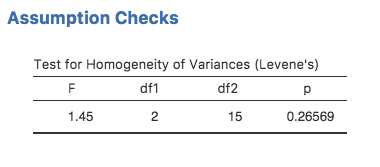
\epsfig{file = ../img/anova/anova4.png, clip=true,width = 10cm}
\caption{Levene test output for one-way ANOVA in jamovi}
\HR
\label{fig:anova4}
\end{center}
\end{figure}

\SUBSECTION{Removing the homogeneity of variance assumption~\label{sec:welchoneway}}

In our example, the homogeneity of variance assumption turned out to be a pretty safe one: the Levene test came back non-significant (notwithstanding that we should also look at the plot of standard deviations), so we probably don't need to worry. However, in real life we aren't always that lucky. How do we save our ANOVA when the homogeneity of variance assumption is violated? If you recall from our discussion of $t$-tests, we've seen this problem before. The Student $t$-test assumes equal variances, so the solution was to use the Welch $t$-test, which does not. In fact, \textcite{Welch1951} also showed how we can solve this problem for ANOVA too (the \keyterm{Welch one-way test}). It's implemented in jamovi using the \rtext{One-Way ANOVA} analysis. This is a specific analysis approach just for one-way ANOVA, and to run the Welch one-way ANOVA for our example, we would re-run the analysis as previously, but this time use the jamovi \rtext{ANOVA - One Way ANOVA} analysis command, and check the option for Welch's test (see Figure \ref{fig:anova4a}.

\begin{figure}[htb]
\begin{center}
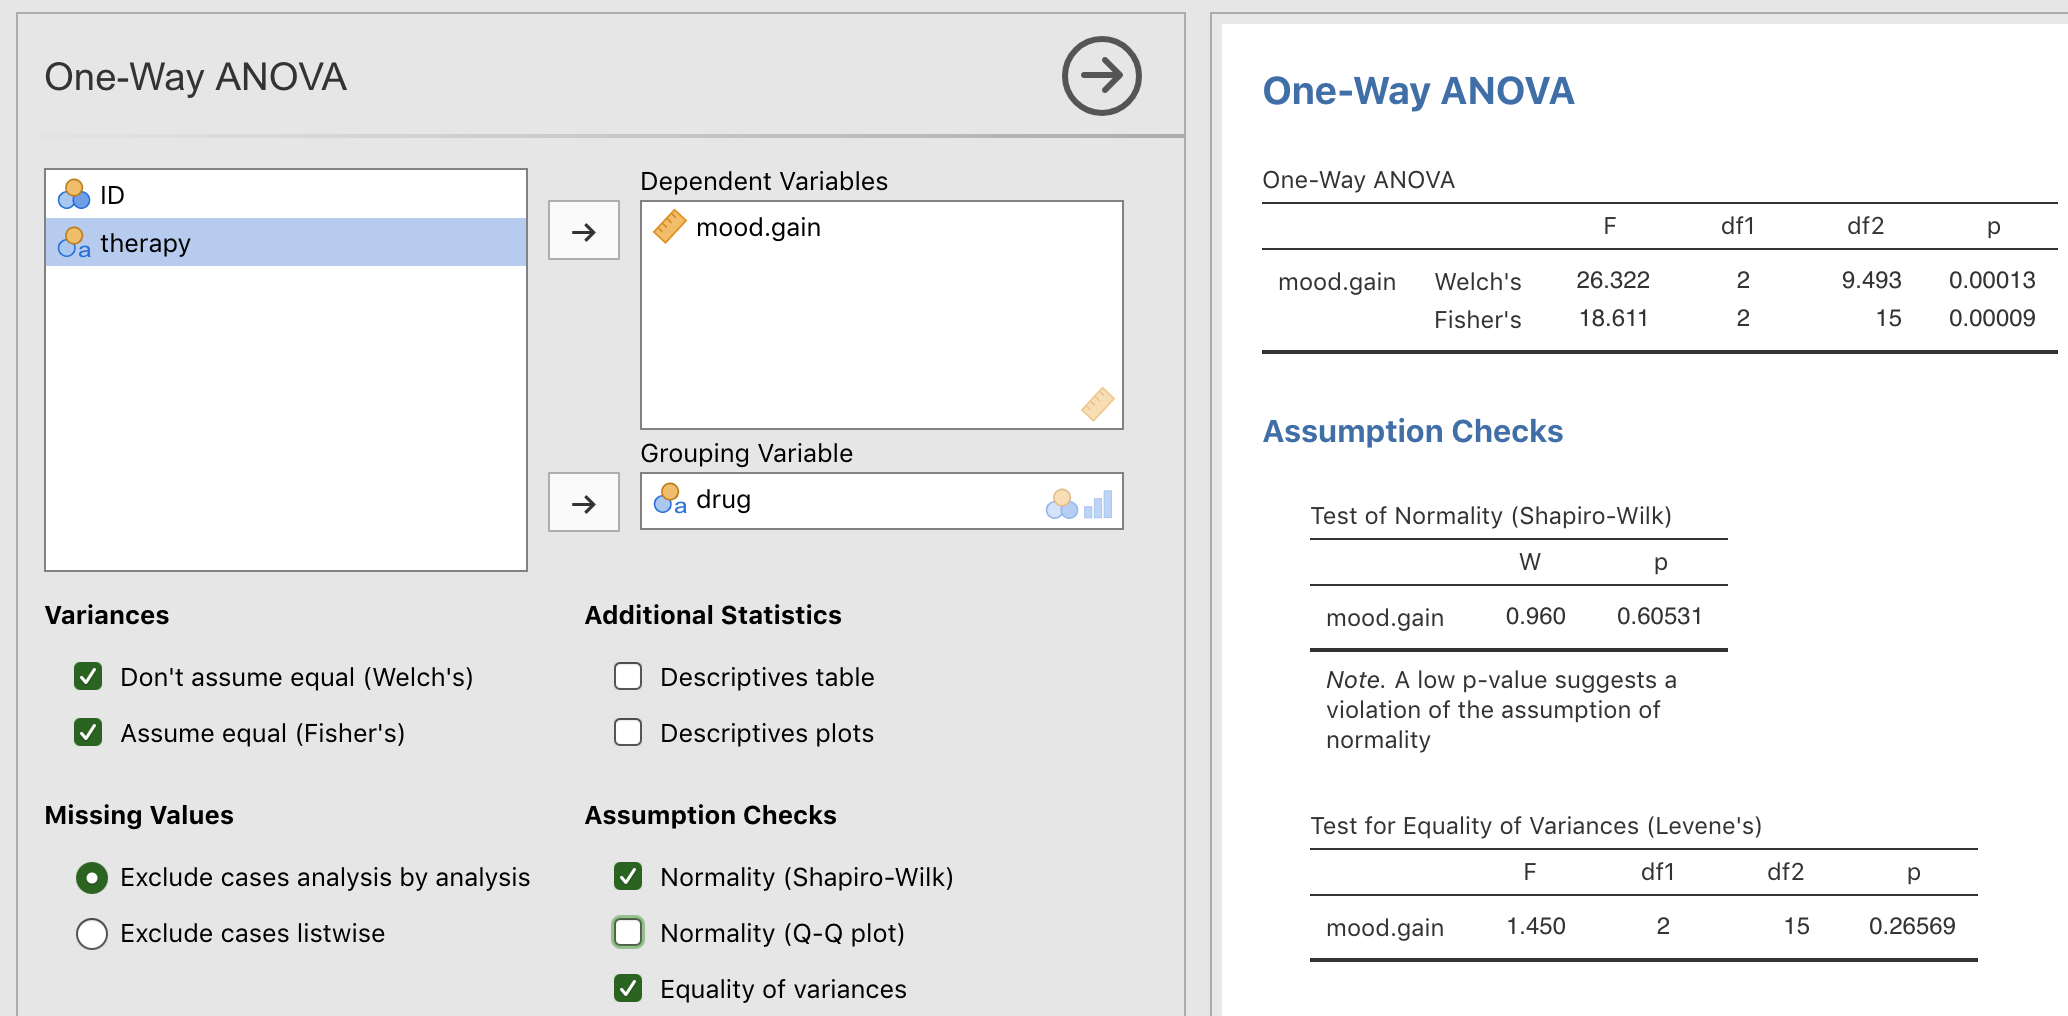
\epsfig{file = ../img/anova/anova4a.png, clip=true,width = 14cm}
\caption{Welch's test as part of the One Way ANOVA analysis in jamovi}
\HR
\label{fig:anova4a}
\end{center}
\end{figure}

\noindent
To understand what's happening here, let's compare these numbers to what we got earlier in Section~\ref{sec:introduceaov} when we ran our original ANOVA. To save you the trouble of flicking back, this is what we got last time: $F(2,15) = 18.611, p=.00009$, also shown as the Fisher's test in the \rtext{One-Way ANOVA} shown in Figure \ref{fig:anova4a}. 

Okay, so originally our ANOVA gave us the result $F(2,15) = 18.6$, whereas the Welch one-way test gave us $F(2,9.49) = 26.32$. In other words, the Welch test has reduced the within-groups degrees of freedom from 15 to 9.49, and the $F$-value has increased from 18.6 to 26.32. 

\SUBSECTION{Checking the normality assumption~\label{sec:anovanormality}}

Testing the normality assumption is relatively straightforward. We covered most of what you need to know in Section~\ref{sec:shapiro}. The only thing we really need to do is draw a QQ plot and, in addition if it is available, run the Shapiro-Wilk test. The QQ plot is shown in Figure~\ref{fig:anova5} and it looks pretty normal to me. If the Shapiro-Wilk test is not significant (i.e. $p<.05$) then this indicates that the assumption of normality is not violated. However, as with Levene's test, if the sample size is large then a significant  Shapiro-Wilk test may in fact be a false positive, where the assumption of normality is not violated in any substantive problematic sense for the analysis. And, similarly, a very small sample can produce false negatives. That's why a visual inspection of the QQ plot is important. 

Alongside inspecting the QQ plot for any deviations from normality, the Shapiro-Wilk test for our data does show a non-significant effect, with $p=0.6053$ (see Figure \ref{fig:anova4a}). This therefore supports the QQ plot assessment; both checks find no indication that normality is violated.

\begin{figure}[p]
\begin{center}
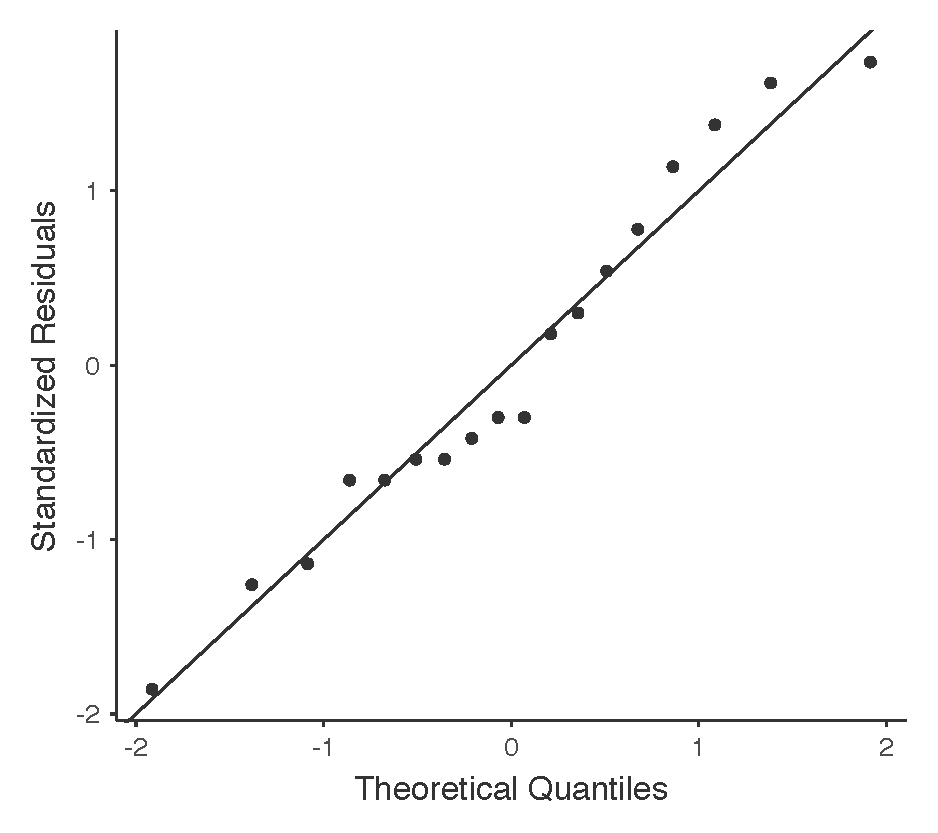
\epsfig{file = ../img/anova/anova5.pdf, clip=true,width = 14cm}
\caption{QQ plot produced from jamovi one way ANOVA options}
\HR
\label{fig:anova5}
\end{center}
\end{figure}


\section{Removing the normality assumption~\label{sec:kruskalwallis}}

Now that we've seen how to check for normality, we are led naturally to ask what we can do to address violations of normality. In the context of a one-way ANOVA, the easiest solution is probably to switch to a non-parametric test (i.e., one that doesn't rely on any particular assumption about the kind of distribution involved). We've seen non-parametric tests before, in Chapter~\ref{ch:ttest}. When you only have two groups, the Mann-Whitney or the Wilcoxon test provides the non-parametric alternative that you need. When you've got three or more groups, you can use the \keyterm{Kruskal-Wallis rank sum test} \parencite{KruskalWallis1952}. So that's the test we'll talk about next.

\SUBSECTION{The logic behind the Kruskal-Wallis test}

The Kruskal-Wallis test is surprisingly similar to ANOVA, in some ways. In ANOVA we started with $Y_{ik}$, the value of the outcome variable for the $i$th person in the $k$th group. For the Kruskal-Wallis test what we'll do is rank order all of these $Y_{ik}$ values and conduct our analysis on the ranked data. 

\vspace{0.7cm}
\begin{mdframed}[style=MyFrame,nobreak=false]
So let's let $R_{ik}$ refer to the ranking given to the $i$th member of the $k$th group. Now, let's calculate $\bar{R}_k$, the average rank given to observations in the $k$th group
$$
\bar{R}_k = \frac{1}{N_K} \sum_{i} R_{ik}
$$
and let's also calculate $\bar{R}$, the grand mean rank
$$
\bar{R} = \frac{1}{N} \sum_{i} \sum_{k} R_{ik}
$$
Now that we've done this, we can calculate the squared deviations from the grand mean rank $\bar{R}$. When we do this for the individual scores, i.e., if we calculate $(R_{ik} - \bar{R})^2$, what we have is a ``nonparametric'' measure of how far the $ik$-th observation deviates from the grand mean rank. When we calculate the squared deviation of the group means from the grand means, i.e., if we calculate $(\bar{R}_k  - \bar{R} )^2$, then what we have is a nonparametric measure of how much the {\it group} deviates from the grand mean rank. With this in mind, we’ll follow the same logic that we did with ANOVA and define our {\it ranked} sums of squares measures, much like we did earlier. First, we have our ``total ranked sums of squares''
$$
\mbox{RSS}_{tot} = \sum_k \sum_i ( R_{ik} - \bar{R} )^2
$$
and we can define the ``between groups ranked sums of squares'' like this
$$
\begin{array}{rcl}
\mbox{RSS}_{b} &=& \sum_k \sum_i ( \bar{R}_k  - \bar{R} )^2 \\
&=& \sum_k N_k ( \bar{R}_k  - \bar{R} )^2 
\end{array}
$$
So, if the null hypothesis is true and there are no true group differences at all, you'd expect the between group rank sums $\mbox{RSS}_{b}$ to be very small, much smaller than the total rank sums $\mbox{RSS}_{tot}$. Qualitatively this is very much the same as what we found when we went about constructing the ANOVA $F$-statistic, but for technical reasons the Kruskal-Wallis test statistic, usually denoted $K$, is constructed in a slightly different way,
$$
K = (N - 1) \times \frac{\mbox{RSS}_b}{\mbox{RSS}_{tot}}
$$
and if the null hypothesis is true, then the sampling distribution of $K$ is {\it approximately} chi-square with $G-1$ degrees of freedom (where $G$ is the number of groups). The larger the value of $K$, the less consistent the data are with the null hypothesis, so this is a one-sided test. We reject $H_0$ when $K$ is sufficiently large.

\SUBSECTION{Additional details}

The description in the previous section illustrates the logic behind the Kruskal-Wallis test. At a conceptual level, this is the right way to think about how the test works. However, from a purely mathematical perspective it's needlessly complicated. I won't show you the derivation, but you can use a bit of algebraic jiggery-pokery\FOOTNOTE{A technical term.} to show that the equation for $K$ can be rewritten as 
$$
K = \frac{12}{N(N-1)} \sum_k N_k {\bar{R}_k}^2    -  3(N+1)
$$
It's this last equation that you sometimes see given for $K$. This is way easier to calculate than the version I described in the previous section, but it's just that it's totally meaningless to actual humans. It's probably best to think of $K$ the way I described it earlier, as an analogue of ANOVA based on ranks. But keep in mind that the test statistic that gets calculated ends up with a rather different look to it than the one we used for our original ANOVA.

But wait, there's more! Dear lord, why is there always {\it more}? The story I've told so far is only actually true when there are no ties in the raw data. That is, if there are no two observations that have exactly the same value. If there {\it are} ties, then we have to introduce a correction factor to these calculations. At this point I'm assuming that even the most diligent reader has stopped caring (or at least formed the opinion that the tie-correction factor is something that doesn't require their immediate attention). So I'll very quickly tell you how it's calculated, and omit the tedious details about {\it why} it's done this way. Suppose we construct a frequency table for the raw data, and let $f_j$ be the number of observations that have the $j$-th unique value. This might sound a bit abstract, so here's a concrete example from the frequency table of \rtext{mood.gain} from the \filename{clinicaltrials.csv} data set:
\begin{rblock1}
0.1 0.2 0.3 0.4 0.5 0.6 0.8 0.9 1.1 1.2 1.3 1.4 1.7 1.8 
  1   1   2   1   1   2   1   1   1   1   2   2   1   1 
\end{rblock1}
Looking at this table, notice that the third entry in the frequency table has a value of $2$. Since this corresponds to a \rtext{mood.gain} of 0.3, this table is telling us that two people's mood increased by 0.3. More to the point, in the mathematical notation I introduced above, this is telling us that $f_3 = 2$. Yay. So, now that we know this, the tie correction factor (TCF) is:
$$
\mbox{TCF} = 1 - \frac{\sum_j {f_j}^3 - f_j}{N^3 - N} 
$$
The tie-corrected value of the Kruskal-Wallis statistic is obtained by dividing the value of $K$ by this quantity. It is this tie-corrected version that jamovi calculates. And at long last, we're actually finished with the theory of the Kruskal-Wallis test. I'm sure you're all terribly relieved that I've cured you of the existential anxiety that naturally arises when you realise that you {\it don't} know how to calculate the tie-correction factor for the Kruskal-Wallis test. Right?
\end{mdframed}


\SUBSECTION{How to run the Kruskal-Wallis test in jamovi} 

Despite the horror that we've gone through in trying to understand what the Kruskal-Wallis test actually does, it turns out that running the test is pretty painless, since jamovi has an analysis as part of the ANOVA analysis set called `Non-Parametric' - `One Way ANOVA (Kruskall-Wallis)' Most of the time you'll have data like the \filename{clinicaltrial.csv} data set, in which you have your outcome variable \rtext{mood.gain} and a grouping variable \rtext{drug}. If so, you can just go ahead and run the analysis in jamovi. What this gives us is a Kruskal-Wallis $\chi^2$ = 12.076, df = 2, $p$-value = 0.00239, as in Figure \ref{fig:anova6}

\vspace{0.5cm}
\begin{figure}[!ht]
\begin{center}
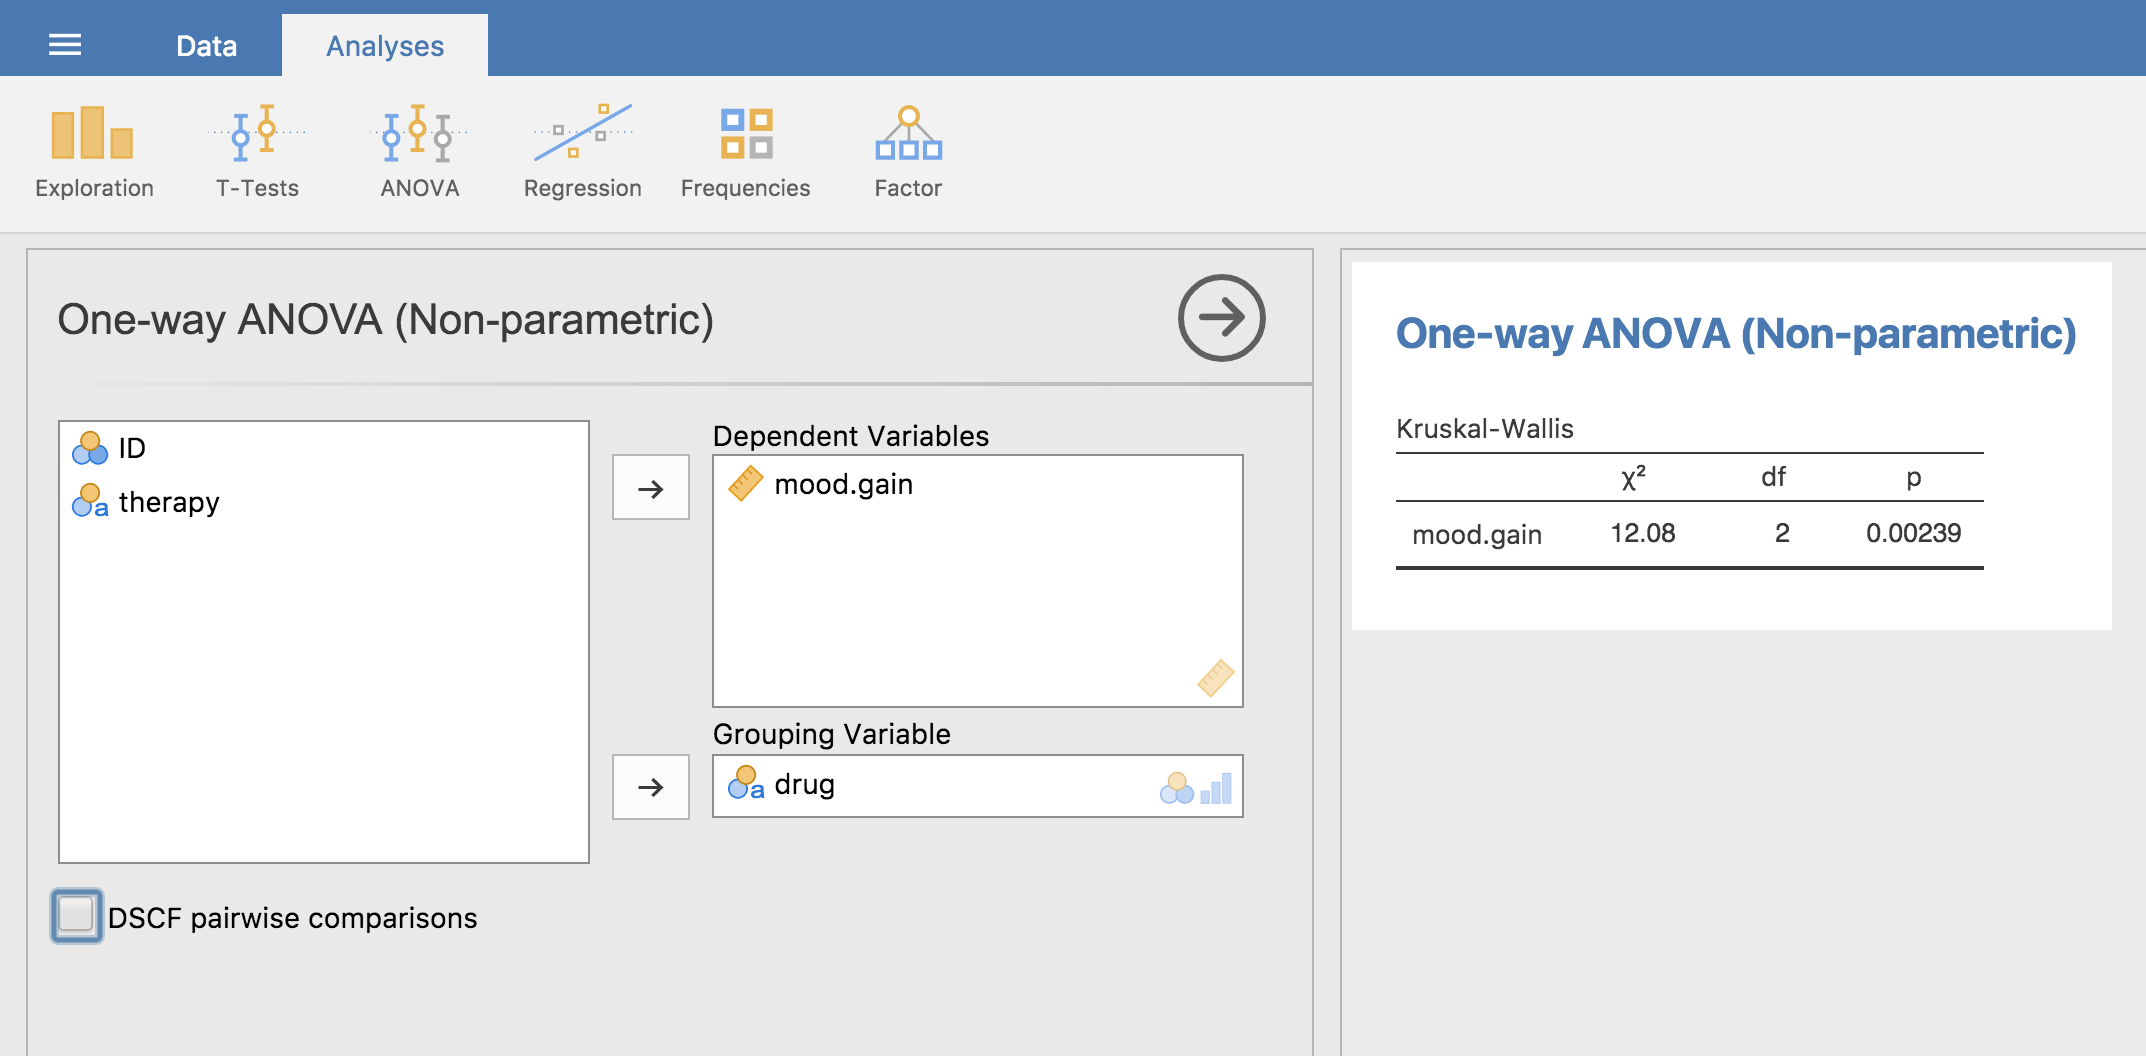
\epsfig{file = ../img/anova/anova6.png, clip=true,width = 14cm}
\caption{Kruskall-Wallis one-way non-parametric ANOVA in jamovi}
\HR
\label{fig:anova6}
\end{center}
\end{figure}

\newpage
\section{Repeated measures one-way ANOVA~\label{sec:RManova}}

The one-way repeated measures ANOVA test is a statistical method of testing for significant differences between three or more groups where the same participants are used in each group (or each participant is closely matched with participants in other experimental groups). For this reason, there should always be an equal number of scores (data points) in each experimental group. This type of design and analysis can also be called a `related ANOVA' or a `within-subjects ANOVA'. 

The logic behind a repeated measures ANOVA is very similar to that of an independent ANOVA (sometimes called a `between-subjects' ANOVA). You'll remember that earlier we showed that in a between-subjects ANOVA total variability is partitioned into between-groups variability ($\mbox{SS}_b$) and within-groups variability ($\mbox{SS}_w$), and after each is divided by the respective degrees of freedom to give $\mbox{MS}_b$ and $\mbox{MS}_w$ (see Table \ref{tab:anovatable}) the $\mbox{F-ratio}$ is calculated as:

\begin{center}
$F = \displaystyle\frac{ \mbox{MS}_b }{ \mbox{MS}_w }$ 
\end{center}

In a repeated measures ANOVA, the $\mbox{F-ratio}$ is calculated in a similar way, but whereas in an independent ANOVA the within-group variability ($\mbox{SS}_w$) is used as the basis for the $\mbox{MS}_w$ denominator, in a repeated measures ANOVA the $\mbox{SS}_w$ is partioned into two parts. As we are using the same subjects in each group, we can remove the variability due to the individual differences between subjects (referred to as $\mbox{SS}_{subjects}$) from the within-groups variability. We won't go into too much technical detail about how this is done, but essentially each subject becomes a level of a factor called subjects. The variability in this within-subjects factor is then calculated in the same way as any between-subjects factor. And then we can subtract $\mbox{SS}_{subjects}$ from $\mbox{SS}_w$ to provide a smaller $\mbox{SS}_{error}$ term: 

\begin{center}
Independent ANOVA: $\mbox{SS}_{error}$ = $\mbox{SS}_w$ \\ \vspace{0.3cm}
Repeated Measures ANOVA: $\mbox{SS}_{error}$ = $\mbox{SS}_w$ - $\mbox{SS}_{subjects}$
\end{center}

This change in $\mbox{SS}_{error}$ term often leads to a more powerful statistical test, but this does depend on whether the reduction in the $\mbox{SS}_{error}$ more than compensates for the reduction in degrees of freedom for the error term (as degrees of freedom go from (n - k)\FOOTNOTE{(n - k) : (number of subjects - number of groups)} to (n - 1)(k - 1) (remembering that there are more subjects in the independent ANOVA design).

\SUBSECTION{Repeated measures ANOVA in jamovi}

First, we need some data. \textcite{Geschwind1972} has suggested that the exact nature of a patient’s language deficit following a stroke can be used to diagnose the specific region of the brain that has been damaged. A researcher is concerned with identifying the specific communication difficulties experienced by six patients suffering from Broca’s Aphasia (a language deficit commonly experienced following a stroke). 

%\vspace{0.5cm}
\begin{table}[!ht]
\caption{Number of attempts successfully completed 
on three experimental tasks.} \label{tab:RManova} \tabcapsep
\begin{center}
\begin{tabular}{c|ccc} 
Participant	& Speech & 	Conceptual & Syntax \\ \hline
1 &	8 &	7 &	6 \\
2 &	7 &	8 &	6 \\
3 &	9 &	5 &	3 \\
4 &	5 &	4 &	5 \\
5 &	6 &	6 &	2 \\
6 &	8 &	7 &	4 \\
\end{tabular}
\tabcapsep \HR
\end{center}
\end{table}

The patients were required to complete three word recognition tasks. On the first (speech production) task, patients were required to repeat single words read out aloud by the researcher. On the second (conceptual) task, designed to test word comprehension, patients were required to match a series of pictures with their correct name. On the third (syntax) task, designed to test knowledge of correct word order, patients were asked to reorder syntactically incorrect sentences. Each patient completed all three tasks. The order in which patients attempted the tasks was counterbalanced between participants. Each task consisted of a series of 10 attempts. The number of attempts successfully completed by each patient are shown in Table \ref{tab:RManova}. Enter these data into jamovi ready for analysis (or take a short-cut and load up the \filename{broca.csv} file). 

To perform a one-way related ANOVA in jamovi, open the one-way repeated measures ANOVA dialogue box, as in Figure \ref{fig:RManova1}, via \rtext{ANOVA - Repeated Measures ANOVA}. Then:
 
\begin{itemize} \itemsep -2pt
\item Enter a Repeated Measures Factor Name. This should be a label that you choose to describe the conditions repeated by all participants. For example, to describe the speech, conceptual and syntax tasks completed by all participants a suitable label would be ‘Task’. Note that this new factor name represents the independent variable in the analysis. 
\item Add a third level in the Repeated Measures Factors text box, as there are three levels representing the three tasks: speech, conceptual and syntax. Change the labels of the levels accordingly.
\item Then move each of the levels variables across to the Repeated Measures Cells text box.
\item Finally, under the Assumption Checks option, tick the “Sphericity checks” text box.
\end{itemize}

\begin{figure}[!htb]
\begin{center}
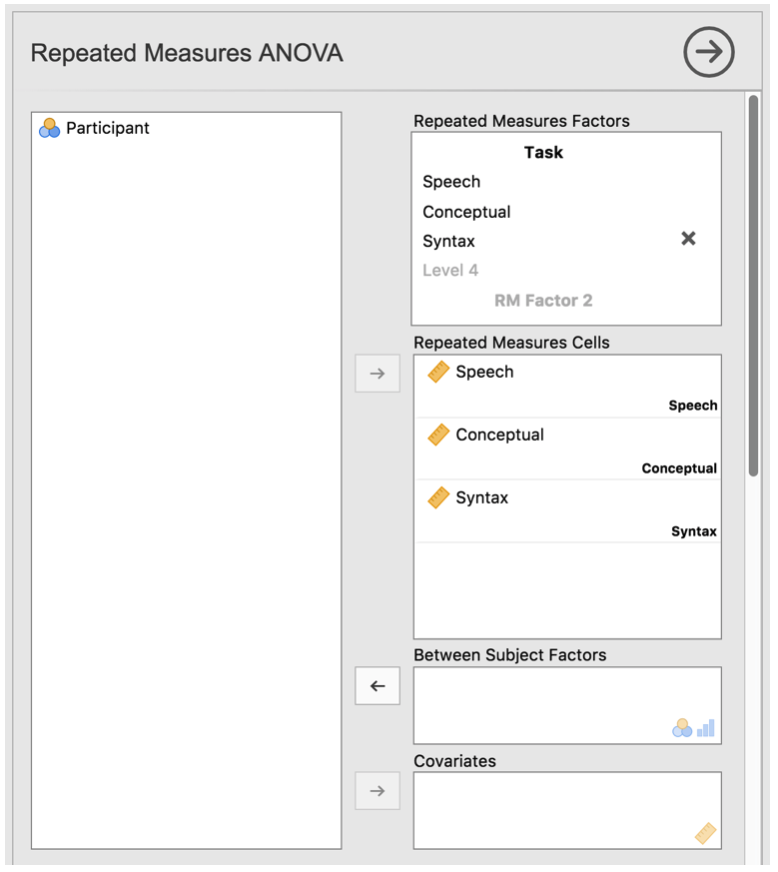
\epsfig{file = ../img/anova/RManova1.png, clip=true,width = 13cm}
\caption{Repeated measures ANOVA dialogue box in jamovi}
\HR
\label{fig:RManova1}
\end{center}
\end{figure}

jamovi output for a one-way repeated measures ANOVA is produced as shown in the Figures \ref{fig:RManova2} to \ref{fig:RManova5}. The first output we should look at is Mauchly’s Test of Sphericity, which tests the hypothesis that the variances of the differences between the conditions are equal (meaning that the spread of difference scores between the study conditions is approximately the same). In Figure \ref{fig:RManova2}, Mauchly’s test significance level is $p=.720$. If Mauchly’s test is non-significant (i.e. $p>.05$, as is the case in this analysis) then it is reasonable to conclude that the variances of the differences are not significantly different (i.e. they are roughly equal and sphericity can be assumed.). 

\begin{figure}[!ht]
\begin{center}
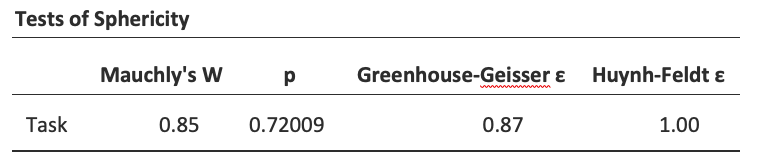
\epsfig{file = ../img/anova/RManova2.png, clip=true,width = 14cm}
\caption{One-way repeated measures ANOVA output: Mauchly’s Test of Sphericity}
\HR
\label{fig:RManova2}
\end{center}
\end{figure}

If, on the other hand, Mauchly’s test had been significant ($p<.05$) then we would conclude that there are significant differences between the variance of the differences, and the requirement of sphericity has not been met. In this case, we should apply a correction to the $F$-value obtained in the one-way related ANOVA analysis: 

\begin{itemize} \itemsep -2pt
\item If the Greenhouse-Geisser value in the “Tests of Sphericity” table is $>.75$ then you should use the Huynh-Feldt correction. 
\item But if the Greenhouse-Geisser value is $<.75$, then you should use the Greenhouse-Geisser correction. 
\end{itemize}

Both these corrected $F$-values can be specified in the Sphericity Corrections check boxes under the Assumption Checks options, and the corrected $F$-values are then shown in the results table, as in Figure \ref{fig:RManova3}.

\begin{figure}[!ht]
\begin{center}
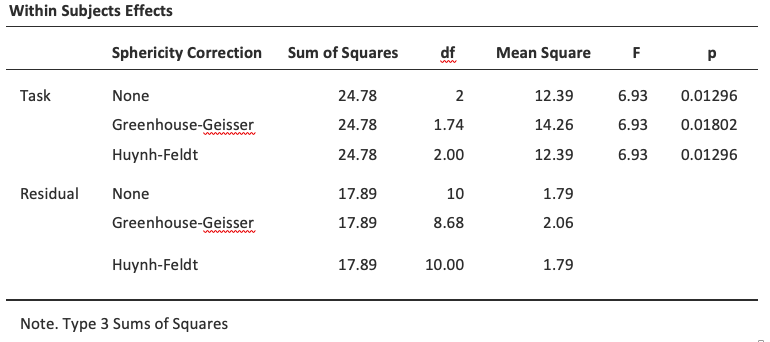
\epsfig{file = ../img/anova/RManova3.png, clip=true,width = 14cm}
\caption{One-way repeated measures ANOVA output: Tests of Within-Subjects Effects}
\HR
\label{fig:RManova3}
\end{center}
\end{figure}

In our analysis, we saw that the significance of Mauchly’s Test of Sphericity was $p=.720$ (i.e. $p>0.05$). So, this means we can assume that the requirement of sphericity has been met so no correction to the $F$-value is needed. Therefore, we can use the ‘None’ Sphericity Correction output values for the repeated measure ‘Task’: $F=6.93, df=2, p=.013$, and we can conclude that the number of tests successfully completed on each language task did vary significantly depending on whether the task was speech, comprehension or syntax based ($F(2,10) = 6.93, p=.013$).

\begin{figure}[!ht]
\begin{center}
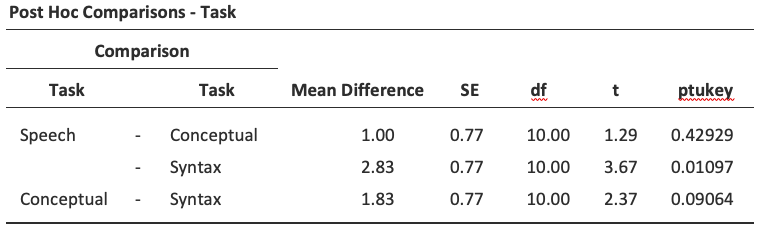
\epsfig{file = ../img/anova/RManova4.png, clip=true,width = 14cm}
\caption{Post-hoc tests in repeated measures ANOVA in jamovi}
\HR
\label{fig:RManova4}
\end{center}
\end{figure}

Post-hoc tests can also be specified in jamovi for repeated measures ANOVA in the same way as for independent ANOVA. The results are shown in Figure \ref{fig:RManova4}. These indicate that there is a significant difference between Speech and Syntax, but not between other levels.

Descriptive statistics (marginal means) can be reviewed to help interpret the results, produced in the jamovi output as in Figure \ref{fig:RManova5}. Comparison of the mean number of trials successfully completed by participants shows that Broca’s Aphasics perform reasonably well on speech production ($mean=7.17$) and language comprehension ($mean=6.17$) tasks. However, their performance was considerably worse on the syntax task ($mean=4.33$), with a significant difference in post-hoc tests between Speech and Syntax task performance. 

\begin{figure}[!ht]
\begin{center}
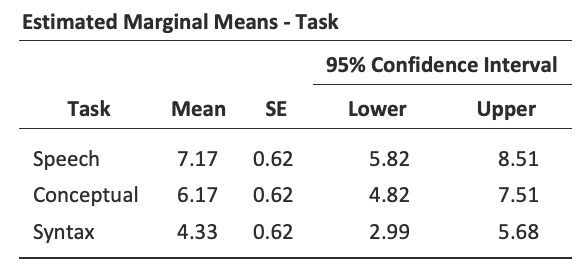
\epsfig{file = ../img/anova/RManova5.png, clip=true,width = 10cm}
\caption{One-way repeated measures ANOVA output: Descriptive Statistics}
\HR
\label{fig:RManova5}
\end{center}
\end{figure}


\section{The Friedman non-parametric repeated measures ANOVA test~\label{sec:Friedman}}

The Friedman test is a non-parametric version of a repeated measures ANOVA and can be used instead of the Kruskall-Wallis test when testing for differences between three or more groups where the same participants are in each group, or each participant is closely matched with participants in other conditions. If the dependent variable is ordinal, or if the assumption of normality is not met, then the Friedman test can be used. 

\vspace{0.5cm}
\begin{figure}[!ht]
\begin{center}
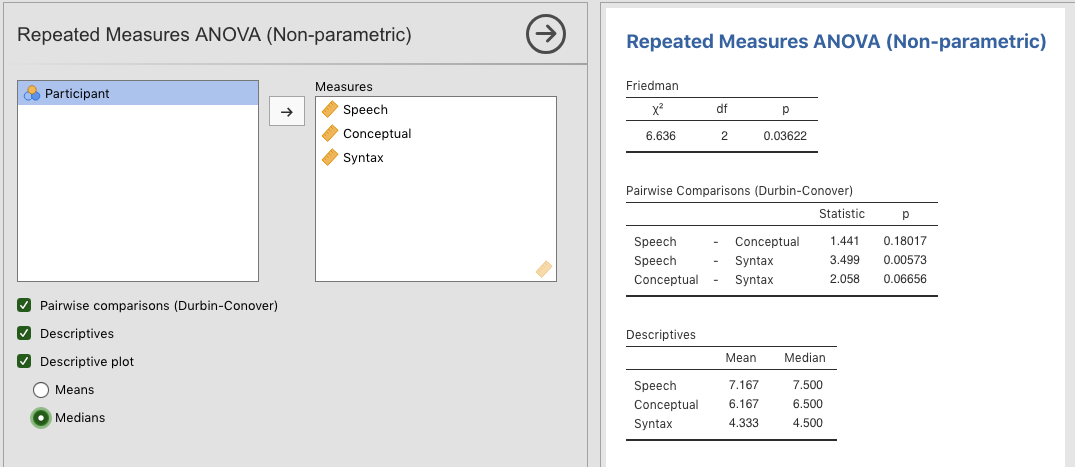
\epsfig{file = ../img/anova/RManova6.png, clip=true,width = 16cm}
\caption{The `Repeated Measures ANOVA (Non-parametric)' dialogue box in jamovi}
\HR
\label{fig:RManova6}
\end{center}
\end{figure}

As with the Kruskall-Wallis test, the underlying mathematics is complicated, and won't be presented here. For the purpose of this book, it is sufficient to note that jamovi calculates the tie-corrected version of the Friedman test, and in Figure \ref{fig:RManova6} there is an example using the Broca's Aphasia data we have already looked at. 

It's pretty straightforward to run a Friedman test in jamovi. Just select \rtext{Analyses - ANOVA - Repeated Measures ANOVA (Non-parametric)}, as in Figure \ref{fig:RManova6}. Then highlight and transfer the names of the repeated measures variables you wish to compare (Speech, Conceptual, Syntax) into the `\rtext{Measures:}'  text box. To produce descriptive statistics (means and medians) for the three repeated measures variables, click on the Descriptives button 

The jamovi results show descriptive statistics, chi-square value, degrees of freedom, and the $p$-value (Figure \ref{fig:RManova6}). Since the $p$-value is less than the level conventionally used to determine significance ($p<.05$), we can conclude that Broca’s Aphasics perform reasonably well on speech production ($median=7.5$) and language comprehension ($median=6.5$) tasks. However, their performance was considerably worse on the syntax task ($median=4.5$), with a significant difference in post-hoc tests between Speech and Syntax task performance. 


\section{On the relationship between ANOVA and the Student \texorpdfstring{\boldm{$t$}}{}-test~\label{sec:anovaandt}}

There's one last thing I want to point out before finishing. It's something that a lot of people find kind of surprising, but it's worth knowing about. An ANOVA with two groups is identical to the Student $t$-test. No, really. It's not just that they are similar, but they are actually equivalent in every meaningful way. I won't try to prove that this is always true, but I will show you a single concrete demonstration. Suppose that, instead of running an ANOVA on our \rtextverb#mood.gain ~ drug# model, let's instead do it using \rtext{therapy} as the predictor. If we run this ANOVA we get an $F$-statistic of  $F(1,16) = 1.71$, and a $p$-value = 0.21. Since we only have two groups, I didn't actually need to resort to an ANOVA, I could have just decided to run a Student $t$-test. So let's see what happens when I do that: I get a $t$-statistic of $t(16) = -1.3068$ and a $p$-value = 0.21. Curiously, the $p$-values are identical. Once again we obtain a value of $p = .21$. But what about the test statistic? Having run a $t$-test instead of an ANOVA, we get a somewhat different answer, namely $t(16) = -1.3068$. However, there is a fairly straightforward relationship here. If we square the $t$-statistic then we get the $F$-statistic from before: $-1.3068^2 = 1.7077$


\section{Summary}

There's a fair bit covered in this chapter, but there's still a lot missing. Most obviously, I haven't discussed how to run an ANOVA when you are interested in more than one grouping variable, but that will be discussed in a lot of detail in Chapter~\ref{ch:anova2}. In terms of what we have discussed, the key topics were:

\begin{itemize} \itemsep -2pt
\item The basic logic behind how ANOVA works (Section~\ref{sec:anovaintro}) and how to run one in jamovi (Section~\ref{sec:introduceaov}).
\item How to compute an effect size for an ANOVA (Section~\ref{sec:etasquared})
\item Post-hoc analysis and corrections for multiple testing (Section~\ref{sec:posthoc}).
\item The assumptions made by ANOVA (Section~\ref{sec:anovaassumptions}).
\item How to check the homogeneity of variance assumption (Section~\ref{sec:levene}) and what to do if it is violated (Section~\ref{sec:welchoneway}).
\item How to check the normality assumption (Section~\ref{sec:anovanormality}) and what to do if it is violated (Section~\ref{sec:kruskalwallis}).
\item Repeated measures ANOVA (Section~\ref{sec:RManova}) and the non-parametric equivalent, the Friedman test (Section \ref{sec:Friedman}).
\end{itemize}

As with all of the chapters in this book, there are quite a few different sources that I've relied upon, but the one stand-out text that I've been most heavily influenced by is \textcite{Sahai2000}. It's not a good book for beginners, but it's an excellent book for more advanced readers who are interested in understanding the mathematics behind ANOVA. 


